\documentclass[11pt,a4paper]{article}

\usepackage[utf8]{inputenc}
\usepackage[T1]{fontenc}
\usepackage{lmodern}
\usepackage[margin=2.5cm,headheight=14pt]{geometry}
\usepackage{graphicx}
\usepackage{booktabs}
\usepackage{amsmath,amssymb}
\usepackage{array}
\usepackage{caption}
\usepackage{fancyhdr}
\usepackage{hyperref}
\usepackage{float}

\hypersetup{
    colorlinks=true,
    linkcolor=black,
    citecolor=black,
    urlcolor=blue
}

\pagestyle{fancy}
\fancyhf{}
\fancyhead[L]{\small Face Attribute Editing in 2D Images}
\fancyhead[R]{\small CS412 Baseline Report}
\fancyfoot[C]{\thepage}
\renewcommand{\headrulewidth}{0.4pt}

\setlength{\parskip}{0.5em}
\setlength{\parindent}{0pt}

\begin{document}

% ---------------------------------------------------------------------------
% Title Page (Matching 23125001_23125006_23125010_Revised_Proposal.pdf)
% ---------------------------------------------------------------------------
\begin{titlepage}
    \centering
    \vspace*{0.5cm}
    
\includegraphics[width=3.6cm]{hcmus_logo.png}\\[0.8cm]

    {\large Vietnam National University, Ho Chi Minh City\\
    Ho Chi Minh City University of Science}\\[1.4cm]

    {\Large \textbf{CS412 - COMPUTER VISION}}\\[0.3cm]
    {\large \textbf{Baseline Reproduction Report}}\\[0.8cm]

    \rule{\textwidth}{0.5pt}\\[0.6cm]
    {\LARGE \textbf{Face Attribute Editing in 2D Images}}\\[0.3cm]
    {\large Learning Adaptive Transport Control for ChordEdit}\\[0.5cm]
    \rule{\textwidth}{0.5pt}\\[1.2cm]

    {\large \textbf{Instructors}}\\[0.2cm]
    {\normalsize Dr. Tran Thai Son and Dr. Vo Hoai Viet}\\[1.0cm]

    {\large \textbf{Project Members}}\\[0.4cm]
    \begin{tabular}{lll}
        \toprule
        \textbf{Student ID} & \textbf{Name} & \textbf{Email} \\
        \midrule
        23125001 & Tang Xuan Bac & \texttt{txbac23@apcs.fitus.edu.vn} \\
        23125006 & Vo Gia Huy    & \texttt{vghuy23@apcs.fitus.edu.vn} \\
        23125010 & Le Dai King   & \texttt{ldking23@apcs.fitus.edu.vn} \\
        \bottomrule
    \end{tabular}

    \vfill
    {\normalsize November 2026}
\end{titlepage}

\setcounter{page}{1}

% ---------------------------------------------------------------------------
% Section 1: Quantitative Results
% ---------------------------------------------------------------------------
\section{Quantitative Results}

\subsection{Experimental Setup and Automatic Evaluators}
We evaluate the original \textbf{ChordEdit} baseline using frozen \textbf{SD-Turbo} weights (Row 1 of Table 2 in our project proposal) across four CelebA facial attribute families: \textbf{Hair Color} (\texttt{black\_to\_blond}, \texttt{brown\_to\_blond}), \textbf{Smiling} (\texttt{add}, \texttt{remove}), \textbf{Eyeglasses} (\texttt{add}, \texttt{remove}), and \textbf{Mustache} (\texttt{add}, \texttt{remove}). All source images are center-cropped and resized to $512 \times 512$ in FP32 precision with random seed $42$ and default transport parameters $(\lambda, \tau) = (1.0, 0.75)$, where $t_{\text{start}} = 0.90$, $\delta = 0.15$, and $t_{\text{end}} = 0.30$. For each of the $120$ held-out test requests ($15$ per editing direction), we evaluate both \textbf{ChordEdit (w/o prox)} (\texttt{cleanup=False}) and \textbf{ChordEdit (w/ prox)} (\texttt{cleanup=True}), yielding $240$ edited test images.
We evaluate the original \textbf{ChordEdit}~\cite{lu2026chordedit,chordedit_repo} baseline using frozen \textbf{SD-Turbo}~\cite{sdturbo} weights across four CelebA~\cite{liu2015celeba,celeba_web} facial attribute families: \textbf{Hair Color} (\texttt{black\_to\_blond}, \texttt{brown\_to\_blond}), \textbf{Smiling} (\texttt{add}, \texttt{remove}), \textbf{Eyeglasses} (\texttt{add}, \texttt{remove}), and \textbf{Mustache} (\texttt{add}, \texttt{remove}). All source images are center-cropped and resized to $512 \times 512$ in FP32 precision with random seed $42$ and default transport parameters $(\lambda, \tau) = (1.0, 0.75)$~\cite{lu2026chordedit,li2026rethinking}, where $t_{\text{start}} = 0.90$, $\delta = 0.15$, and $t_{\text{end}} = 0.30$. For each of the $120$ held-out test requests ($15$ per editing direction), we evaluate both \textbf{ChordEdit (w/o prox)} (\texttt{cleanup=False}) and \textbf{ChordEdit (w/ prox)} (\texttt{cleanup=True}), yielding $240$ edited test images.

Following Section 6.1 of the revised proposal, we report two automatic measurements:
\begin{enumerate}
    \item \textbf{Attribute correctness:} A frozen CLIP-based facial-attribute classifier trained on the official CelebA training partition (\texttt{partition=0}) predicts the target state for \texttt{Blond\_Hair}, \texttt{Smiling}, \texttt{Eyeglasses}, and \texttt{Mustache}. Its decision thresholds $\theta$ are fixed after verifying agreement with ground-truth source labels on the $80$-image validation split (Table~\ref{tab:val_agreement}).
    \item \textbf{Identity preservation:} A frozen ArcFace recognition model (\texttt{buffalo\_l / w600k\_r50}) computes source--output cosine similarity on unit-normalized aligned-face embeddings:
    \item \textbf{Attribute correctness:} A frozen CLIP-based~\cite{radford2021clip} facial-attribute classifier trained on the official CelebA training partition (\texttt{partition=0})~\cite{liu2015celeba} predicts the target state for \texttt{Blond\_Hair}, \texttt{Smiling}, \texttt{Eyeglasses}, and \texttt{Mustache}. Its decision thresholds $\theta$ are fixed after verifying agreement with ground-truth source labels on the $80$-image validation split (Table~\ref{tab:val_agreement}).
    \item \textbf{Identity preservation:} A frozen ArcFace-compatible recognition model (\texttt{buffalo\_l / w600k\_r50})~\cite{deng2019arcface} computes source--output cosine similarity on unit-normalized aligned-face embeddings:
    \begin{equation}
        s_{\text{id}}(x, y) = \phi(x)^\top \phi(y).
    \end{equation}
    Face detection failures are tracked and reported separately rather than silently excluded.
\end{enumerate}

\begin{table}[H]
\centering
\caption{Validation source-label agreement and fixed classifier thresholds on the 80 validation requests.}
\label{tab:val_agreement}
\begin{tabular}{lcc}
\toprule
\textbf{Target Attribute} & \textbf{Validation Agreement (\%)} & \textbf{Fixed Threshold ($\theta$)} \\
\midrule
\texttt{Blond\_Hair} & 91.25\% & 0.590 \\
\texttt{Smiling}     & 95.00\% & 0.400 \\
\texttt{Eyeglasses}  & 98.75\% & 0.300 \\
\texttt{Mustache}    & 95.00\% & 0.570 \\
\bottomrule
\end{tabular}
\end{table}

\subsection{Baseline Automatic Measurements on Held-Out Test Set}
Table~\ref{tab:quant_results} summarizes automatic target-attribute success, mean target confidence, ArcFace cosine similarity $s_{\text{id}}$, face detection failures, and per-image inference latency (on a single NVIDIA Tesla T4 GPU) across all eight editing directions.

\begin{table}[H]
\centering
\caption{Automatic evaluation of the Original ChordEdit baseline on the held-out CelebA test set ($120$ requests $\times$ $2$ refinement conditions $= 240$ outputs).}
\label{tab:quant_results}
\vspace{0.15cm}
\resizebox{\textwidth}{!}{%
\begin{tabular}{llclcccc}
\toprule
\textbf{Attribute} & \textbf{Direction} & \textbf{$N$} & \textbf{Method} & \textbf{Attr. Succ.} & \textbf{Target Conf.} & \textbf{ArcFace $s_{\text{id}}$} & \textbf{Det. Fail} \\
\midrule
Hair\_Color & \texttt{black\_to\_blond} & 15 & ChordEdit (w/o prox) &  0.0\% & 0.093 & 0.612 & 0/15 \\
Hair\_Color & \texttt{black\_to\_blond} & 15 & ChordEdit (w/ prox)  & 33.3\% & 0.333 & 0.280 & 0/15 \\
\addlinespace[2pt]
Hair\_Color & \texttt{brown\_to\_blond} & 15 & ChordEdit (w/o prox) & 46.7\% & 0.496 & 0.689 & 0/15 \\
Hair\_Color & \texttt{brown\_to\_blond} & 15 & ChordEdit (w/ prox)  & 60.0\% & 0.648 & 0.330 & 0/15 \\
\midrule
Smiling     & \texttt{add}              & 15 & ChordEdit (w/o prox) & 93.3\% & 0.872 & 0.515 & 0/15 \\
Smiling     & \texttt{add}              & 15 & ChordEdit (w/ prox)  & 100.0\% & 0.983 & 0.213 & 0/15 \\
\addlinespace[2pt]
Smiling     & \texttt{remove}           & 15 & ChordEdit (w/o prox) & 53.3\% & 0.552 & 0.570 & 0/15 \\
Smiling     & \texttt{remove}           & 15 & ChordEdit (w/ prox)  & 66.7\% & 0.635 & 0.281 & 0/15 \\
\midrule
Eyeglasses  & \texttt{add}              & 15 & ChordEdit (w/o prox) & 93.3\% & 0.881 & 0.632 & 0/15 \\
Eyeglasses  & \texttt{add}              & 15 & ChordEdit (w/ prox)  & 93.3\% & 0.921 & 0.286 & 0/15 \\
\addlinespace[2pt]
Eyeglasses  & \texttt{remove}           & 15 & ChordEdit (w/o prox) &  0.0\% & 0.008 & 0.665 & 0/15 \\
Eyeglasses  & \texttt{remove}           & 15 & ChordEdit (w/ prox)  &  0.0\% & 0.009 & 0.299 & 0/15 \\
\midrule
Mustache    & \texttt{add}              & 15 & ChordEdit (w/o prox) & 86.7\% & 0.815 & 0.741 & 0/15 \\
Mustache    & \texttt{add}              & 15 & ChordEdit (w/ prox)  & 86.7\% & 0.851 & 0.361 & 1/15 \\
\addlinespace[2pt]
Mustache    & \texttt{remove}           & 15 & ChordEdit (w/o prox) & 26.7\% & 0.228 & 0.742 & 0/15 \\
Mustache    & \texttt{remove}           & 15 & ChordEdit (w/ prox)  & 66.7\% & 0.500 & 0.424 & 0/15 \\
\midrule
\textbf{Overall} & \textbf{All 8 Directions} & \textbf{120} & \textbf{ChordEdit (w/o prox)} & \textbf{50.0\%} & \textbf{0.493} & \textbf{0.646} & \textbf{0/120} \\
\textbf{Overall} & \textbf{All 8 Directions} & \textbf{120} & \textbf{ChordEdit (w/ prox)}  & \textbf{63.3\%} & \textbf{0.610} & \textbf{0.309} & \textbf{1/120} \\
\bottomrule
\end{tabular}%
}
\end{table}

\textbf{Key Quantitative Observations:}
\begin{itemize}
    \item \textbf{Effect of Proximal Refinement (RQ3):} Enabling proximal refinement (\texttt{w/ prox}) increases overall target-attribute success from \textbf{50.0\%} to \textbf{63.3\%} ($+13.3\%$ absolute gain, with mean target confidence rising from $0.493$ to $0.610$), with strong improvements on \texttt{Mustache/remove} ($26.7\% \to 66.7\%$) and \texttt{Hair\_Color/black\_to\_blond} ($0.0\% \to 33.3\%$). However, this comes at a clear cost to biometric identity preservation: mean ArcFace similarity drops from \textbf{0.646} (\texttt{w/o prox}) to \textbf{0.309} (\texttt{w/ prox}), alongside a modest $+11.9\%$ runtime overhead ($2.819\,\text{s}$ vs.\ $3.154\,\text{s}$ per image on Tesla T4).
    \item \textbf{Task Asymmetry and Need for Adaptive Control (RQ1 \& RQ2):} Under the fixed default $(\lambda, \tau) = (1.0, 0.75)$, attribute addition tasks (\texttt{Smiling/add}: $93.3\%\text{--}100\%$, \texttt{Eyeglasses/add}: $93.3\%$, \texttt{Mustache/add}: $86.7\%$) succeed reliably, whereas removal tasks (\texttt{Eyeglasses/remove}: $0.0\%$) and dark-to-blond hair edits struggle or suffer identity drift, motivating an input-conditioned transport controller.
\end{itemize}

% ---------------------------------------------------------------------------
% Section 2: Qualitative Results (8 Full-Page Figures)
% ---------------------------------------------------------------------------
\section{Qualitative Results}

Figures~\ref{fig:hair_black}--\ref{fig:mustache_remove} present full-page qualitative comparisons across all eight editing prompts on the held-out test set. Each figure displays four test portraits arranged in three columns: \textbf{Original}, \textbf{ChordEdit (w/o prox)}, and \textbf{ChordEdit (w/ prox)}. Without proximal refinement (\texttt{w/o prox}), the one-step linear latent update preserves coarse facial geometry ($s_{\text{id}} = 0.646$) but introduces off-manifold color blotches around edited regions (mouth, eyes, and hairline). Enabling proximal refinement (\texttt{w/ prox}) projects the edited latent back onto the natural face manifold, eliminating high-frequency artifacts and sharpening the target attribute, though sometimes altering fine facial identity features when $\lambda = 1.0$ is overly aggressive.

\clearpage

\begin{figure}[p]
    \centering
    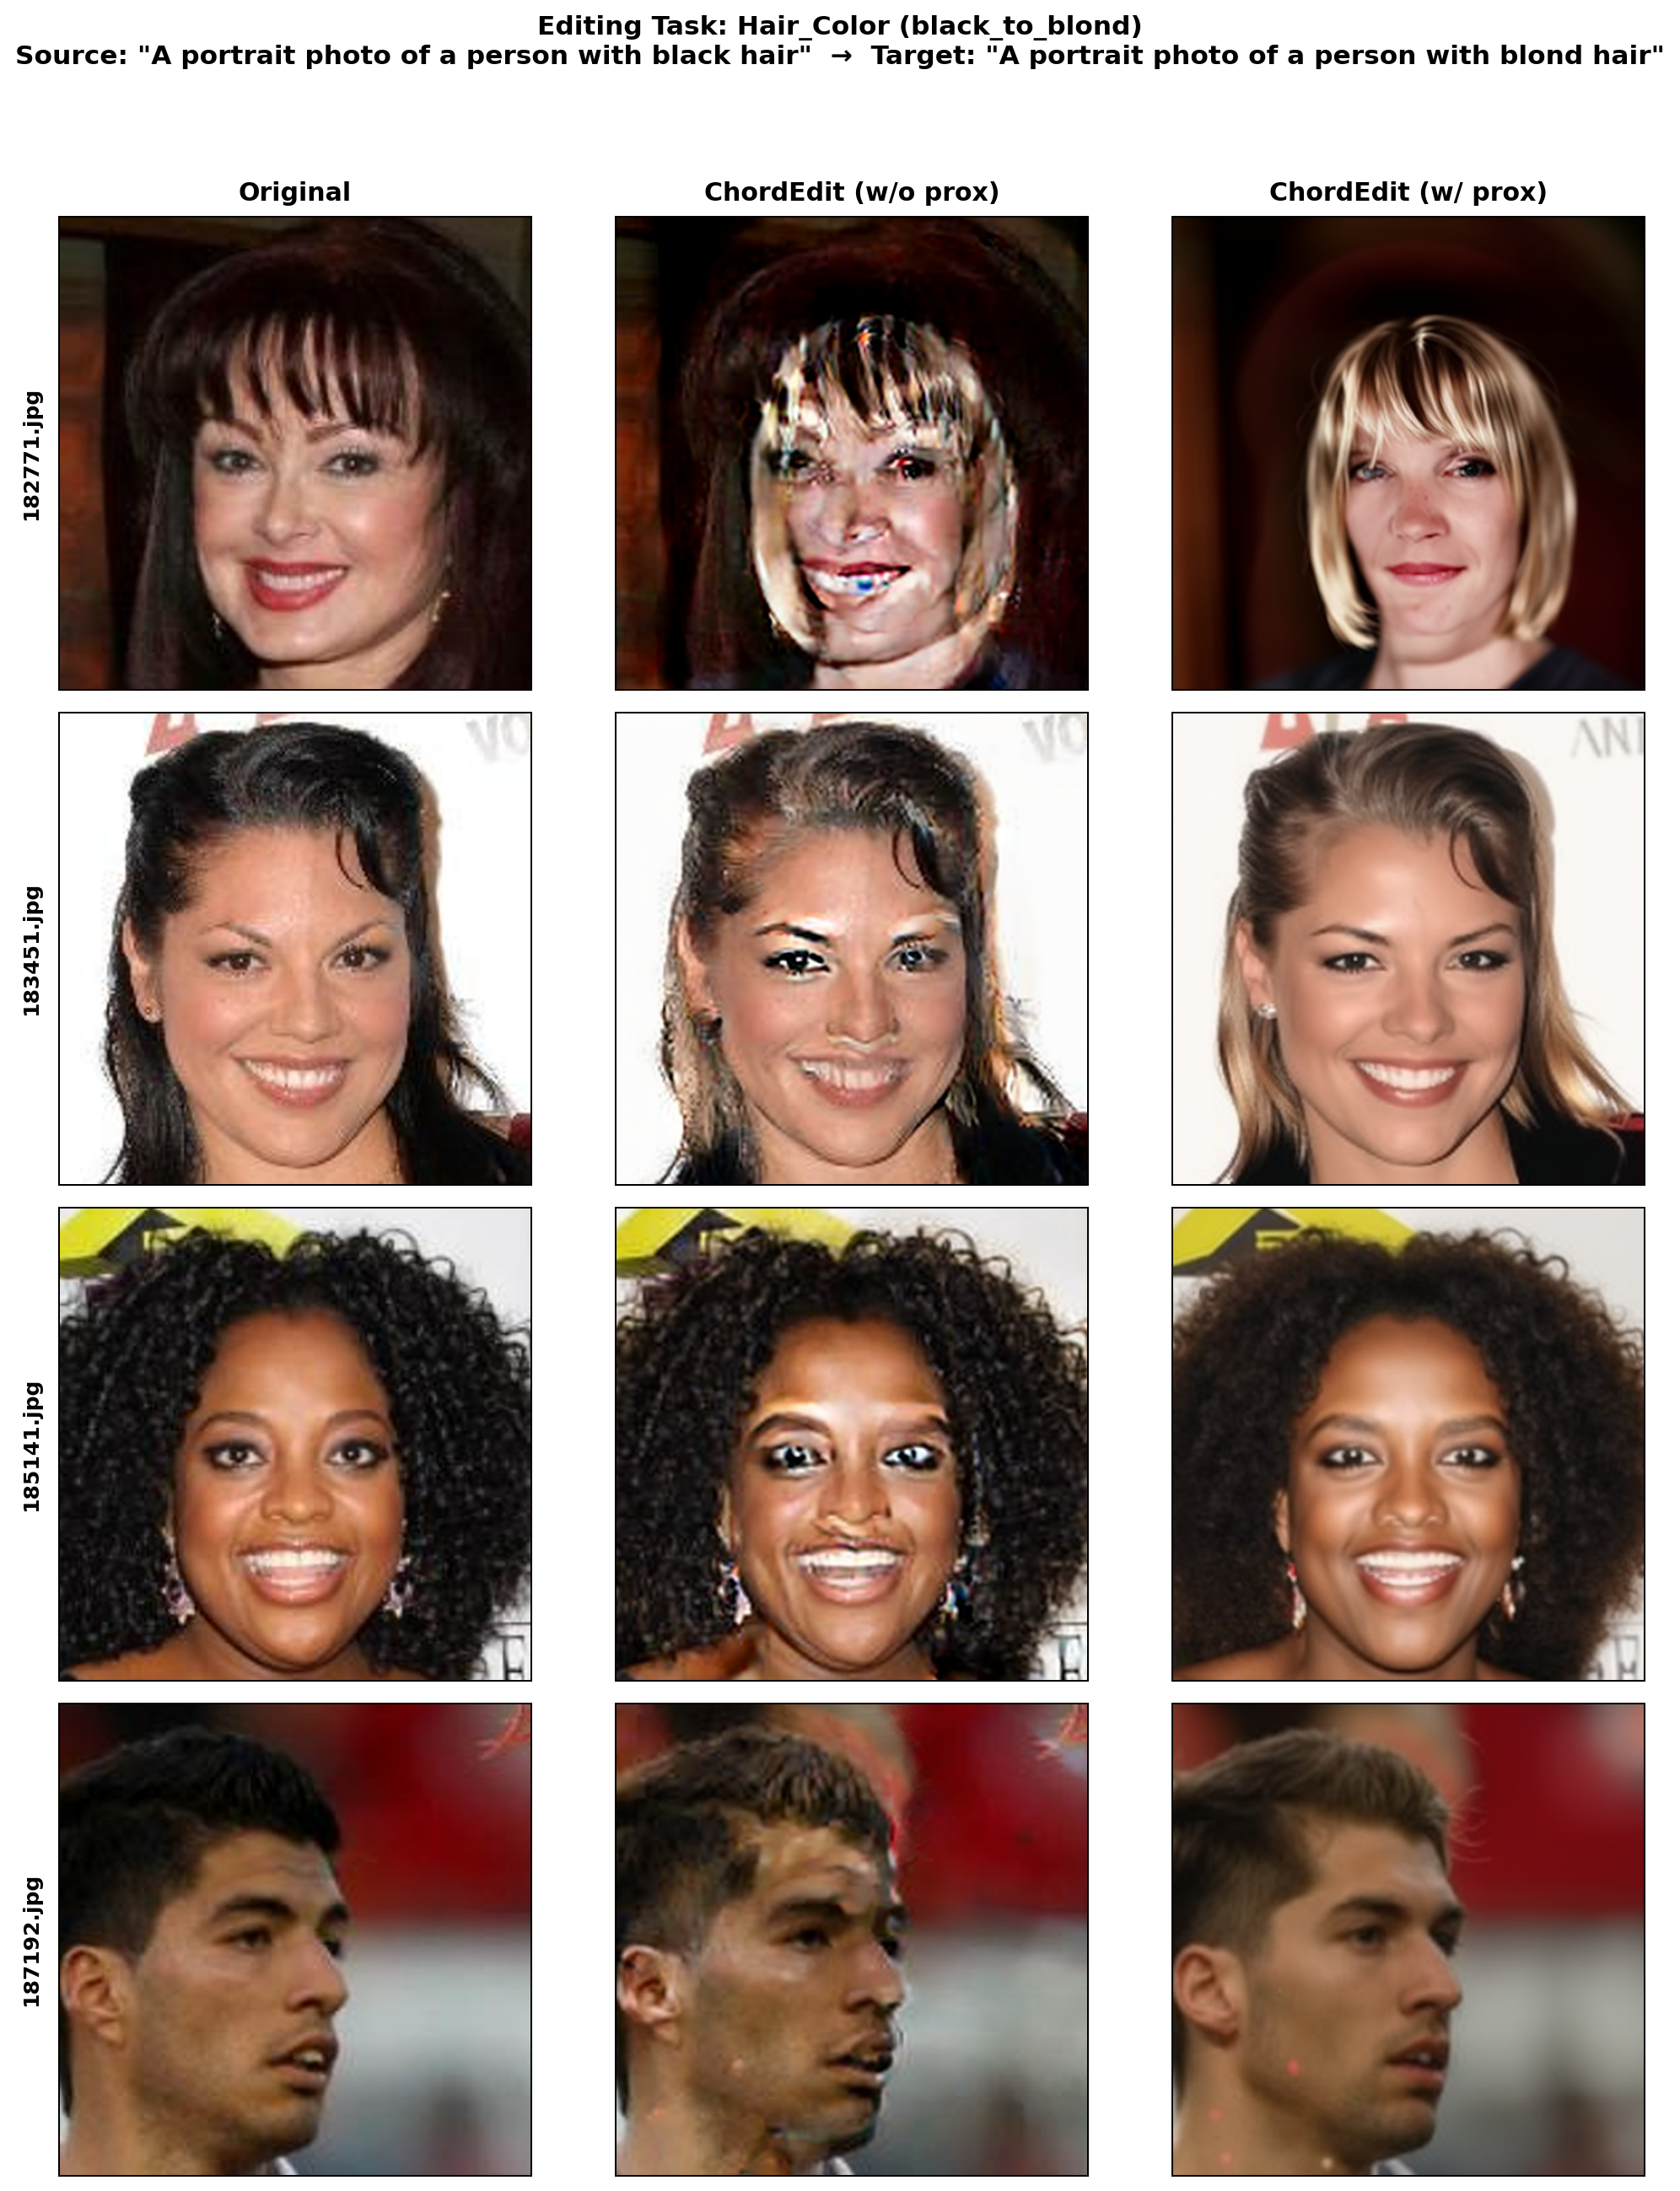
\includegraphics[width=0.95\textwidth,height=0.82\textheight,keepaspectratio]{figures/figure_hair_color_black_to_blond.png}
    \caption{Qualitative baseline results for \textbf{Hair Color (\texttt{black\_to\_blond})}: comparing Original, ChordEdit (w/o prox), and ChordEdit (w/ prox).}
    \label{fig:hair_black}
\end{figure}

\begin{figure}[p]
    \centering
    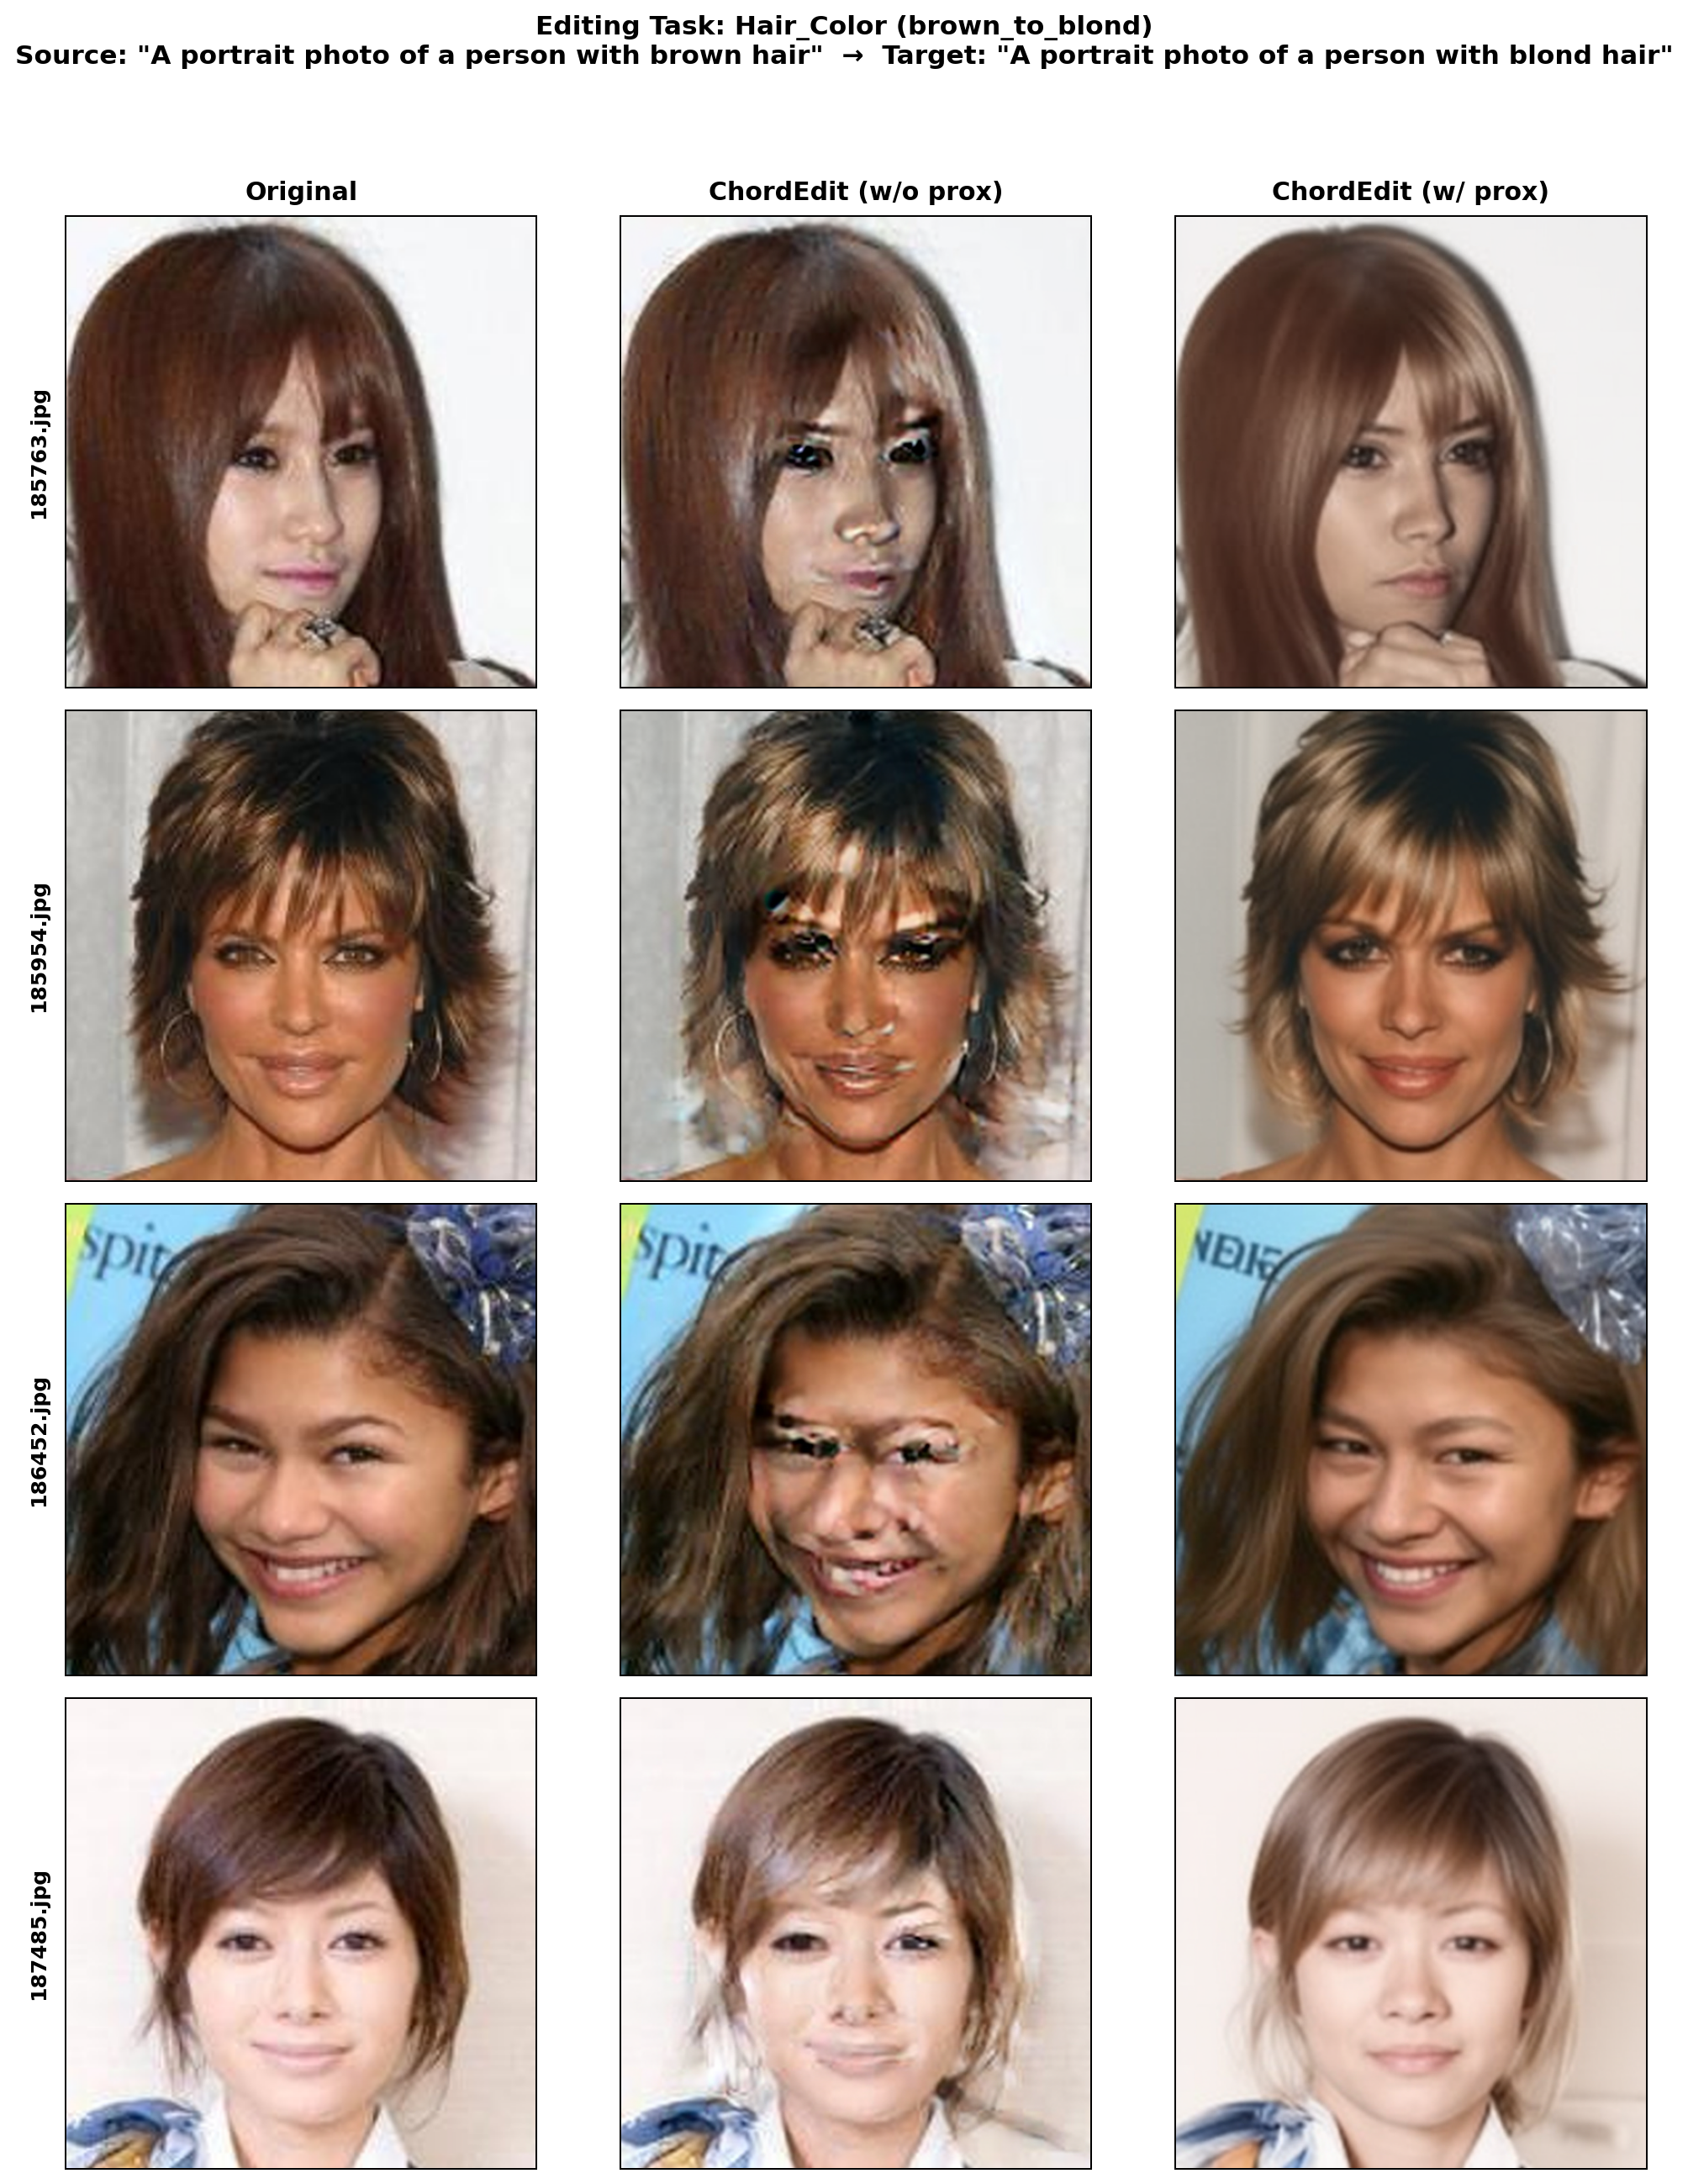
\includegraphics[width=0.95\textwidth,height=0.86\textheight,keepaspectratio]{figures/figure_hair_color_brown_to_blond.png}
    \caption{Qualitative baseline results for \textbf{Hair Color (\texttt{brown\_to\_blond})}: comparing Original, ChordEdit (w/o prox), and ChordEdit (w/ prox).}
    \label{fig:hair_brown}
\end{figure}

\begin{figure}[p]
    \centering
    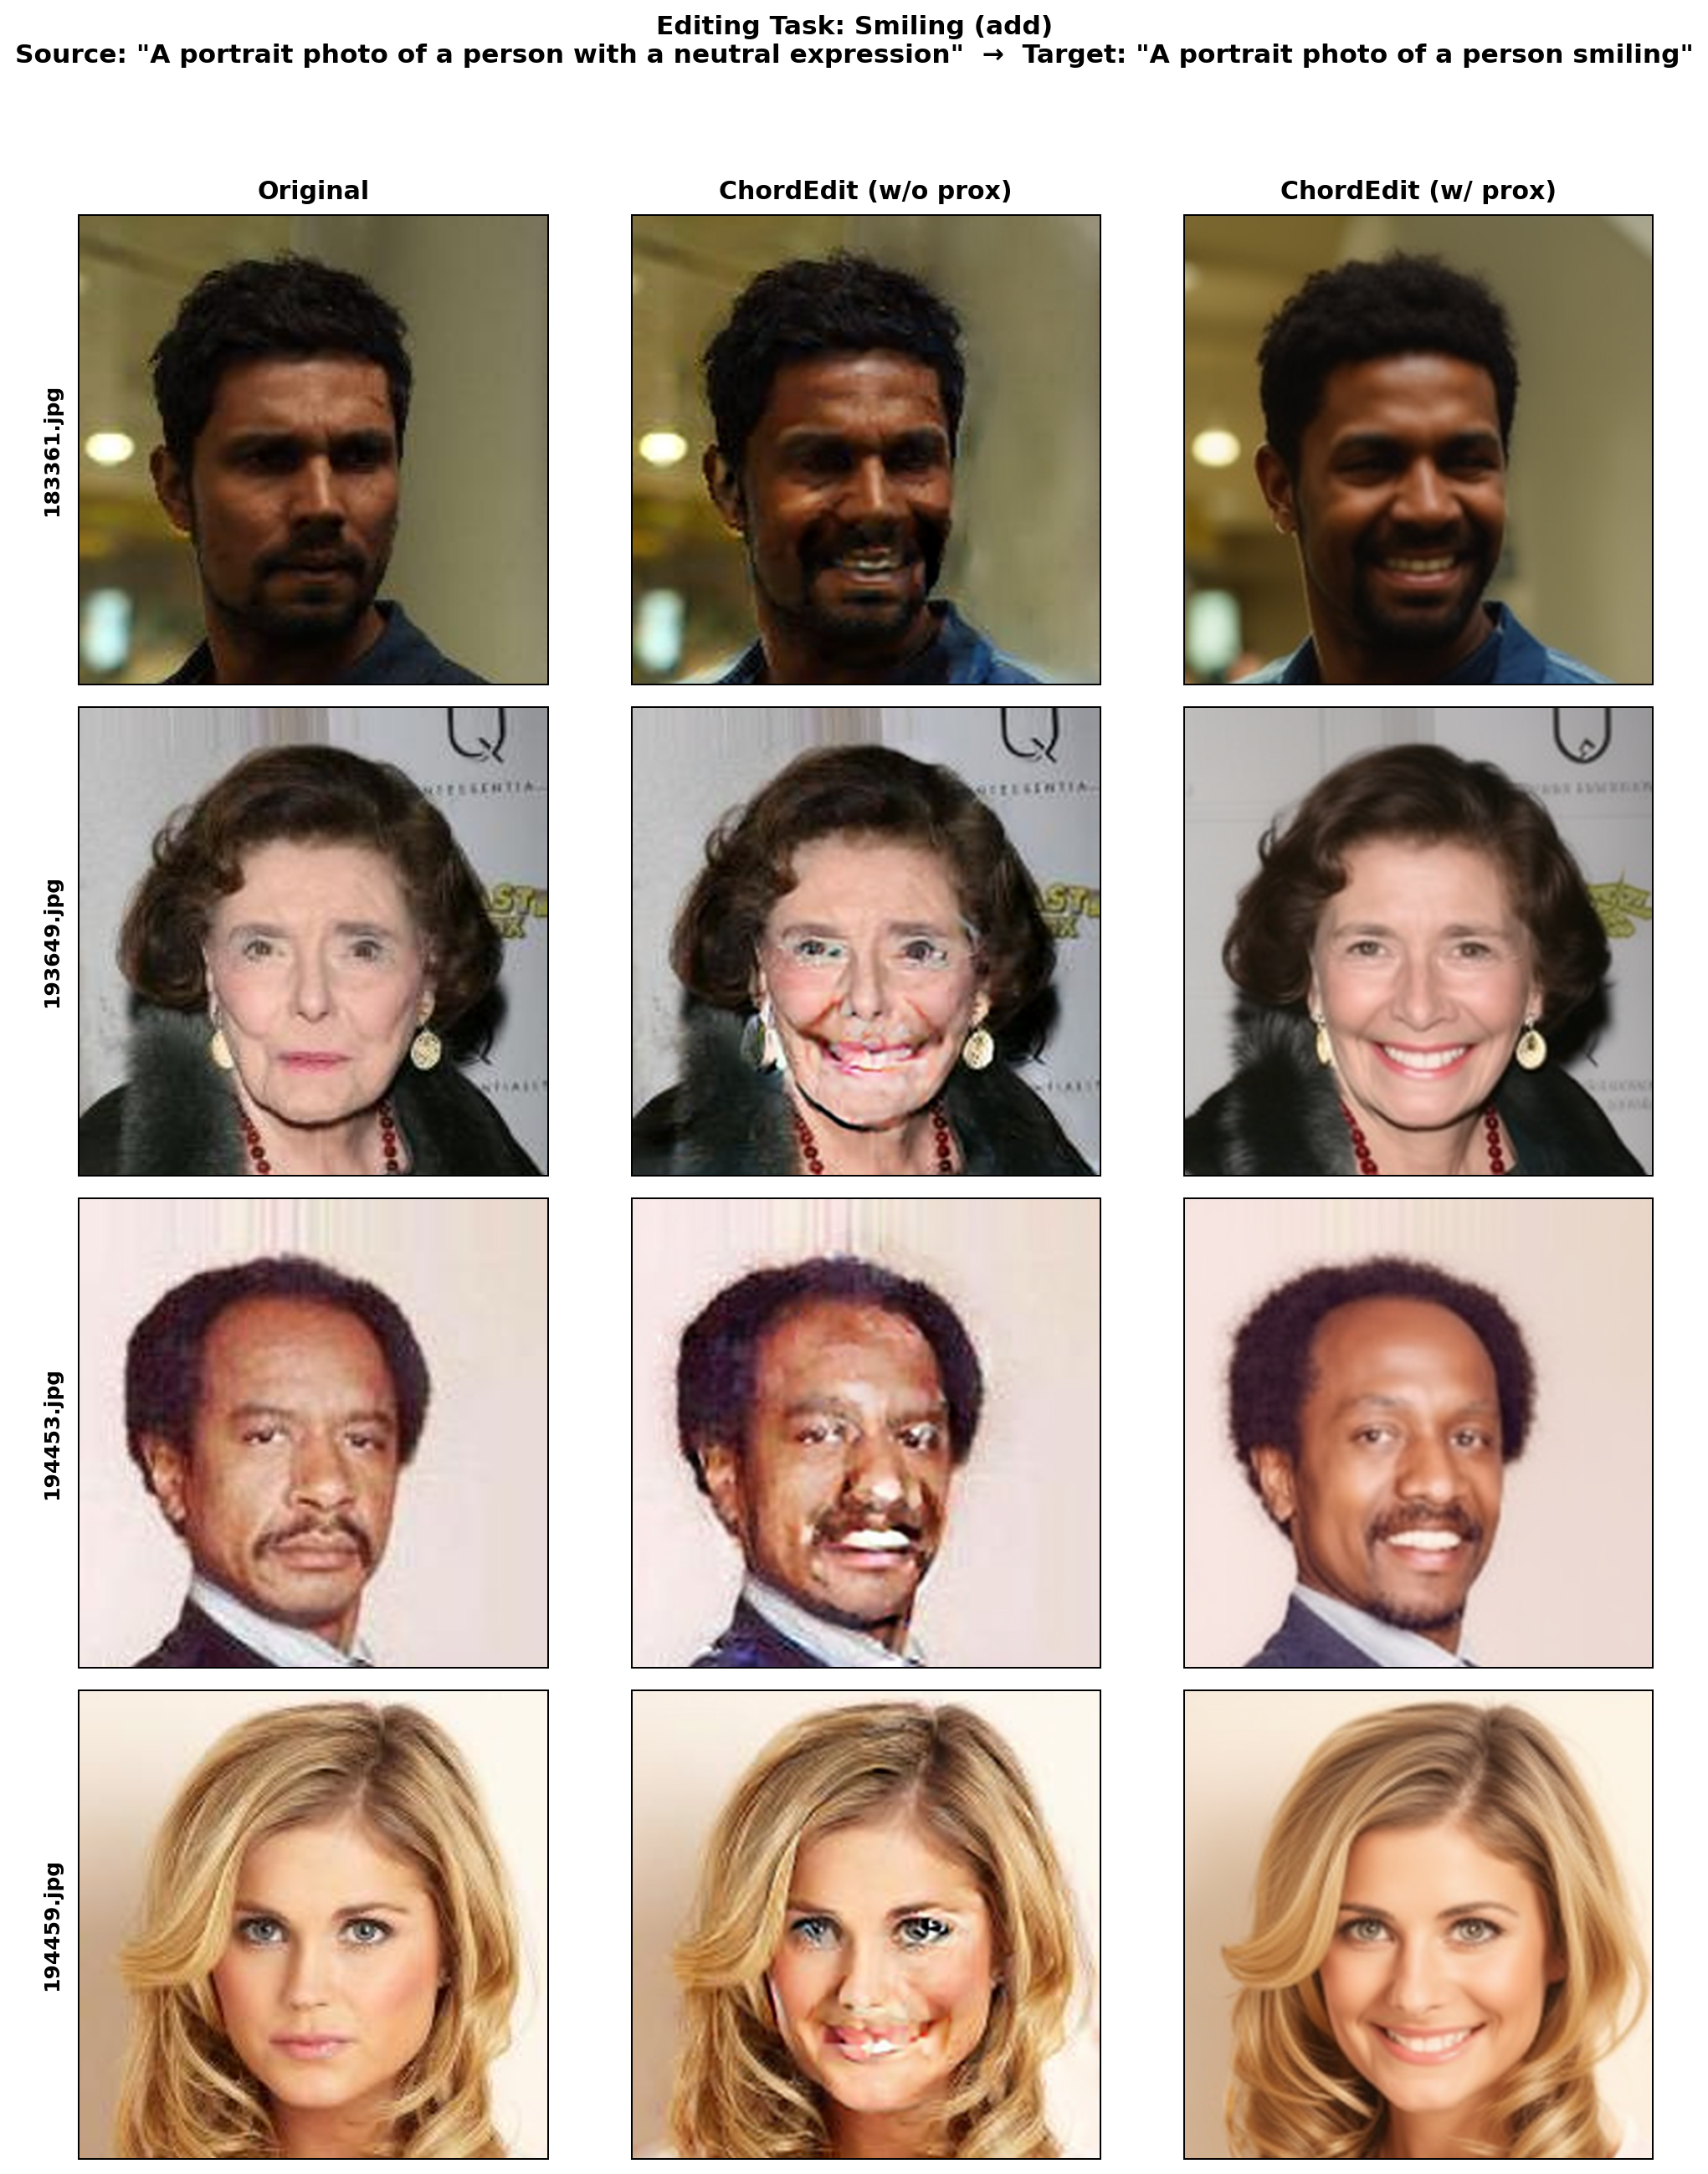
\includegraphics[width=0.95\textwidth,height=0.86\textheight,keepaspectratio]{figures/figure_smiling_add.png}
    \caption{Qualitative baseline results for \textbf{Smiling (\texttt{add})}: comparing Original, ChordEdit (w/o prox), and ChordEdit (w/ prox).}
    \label{fig:smiling_add}
\end{figure}

\begin{figure}[p]
    \centering
    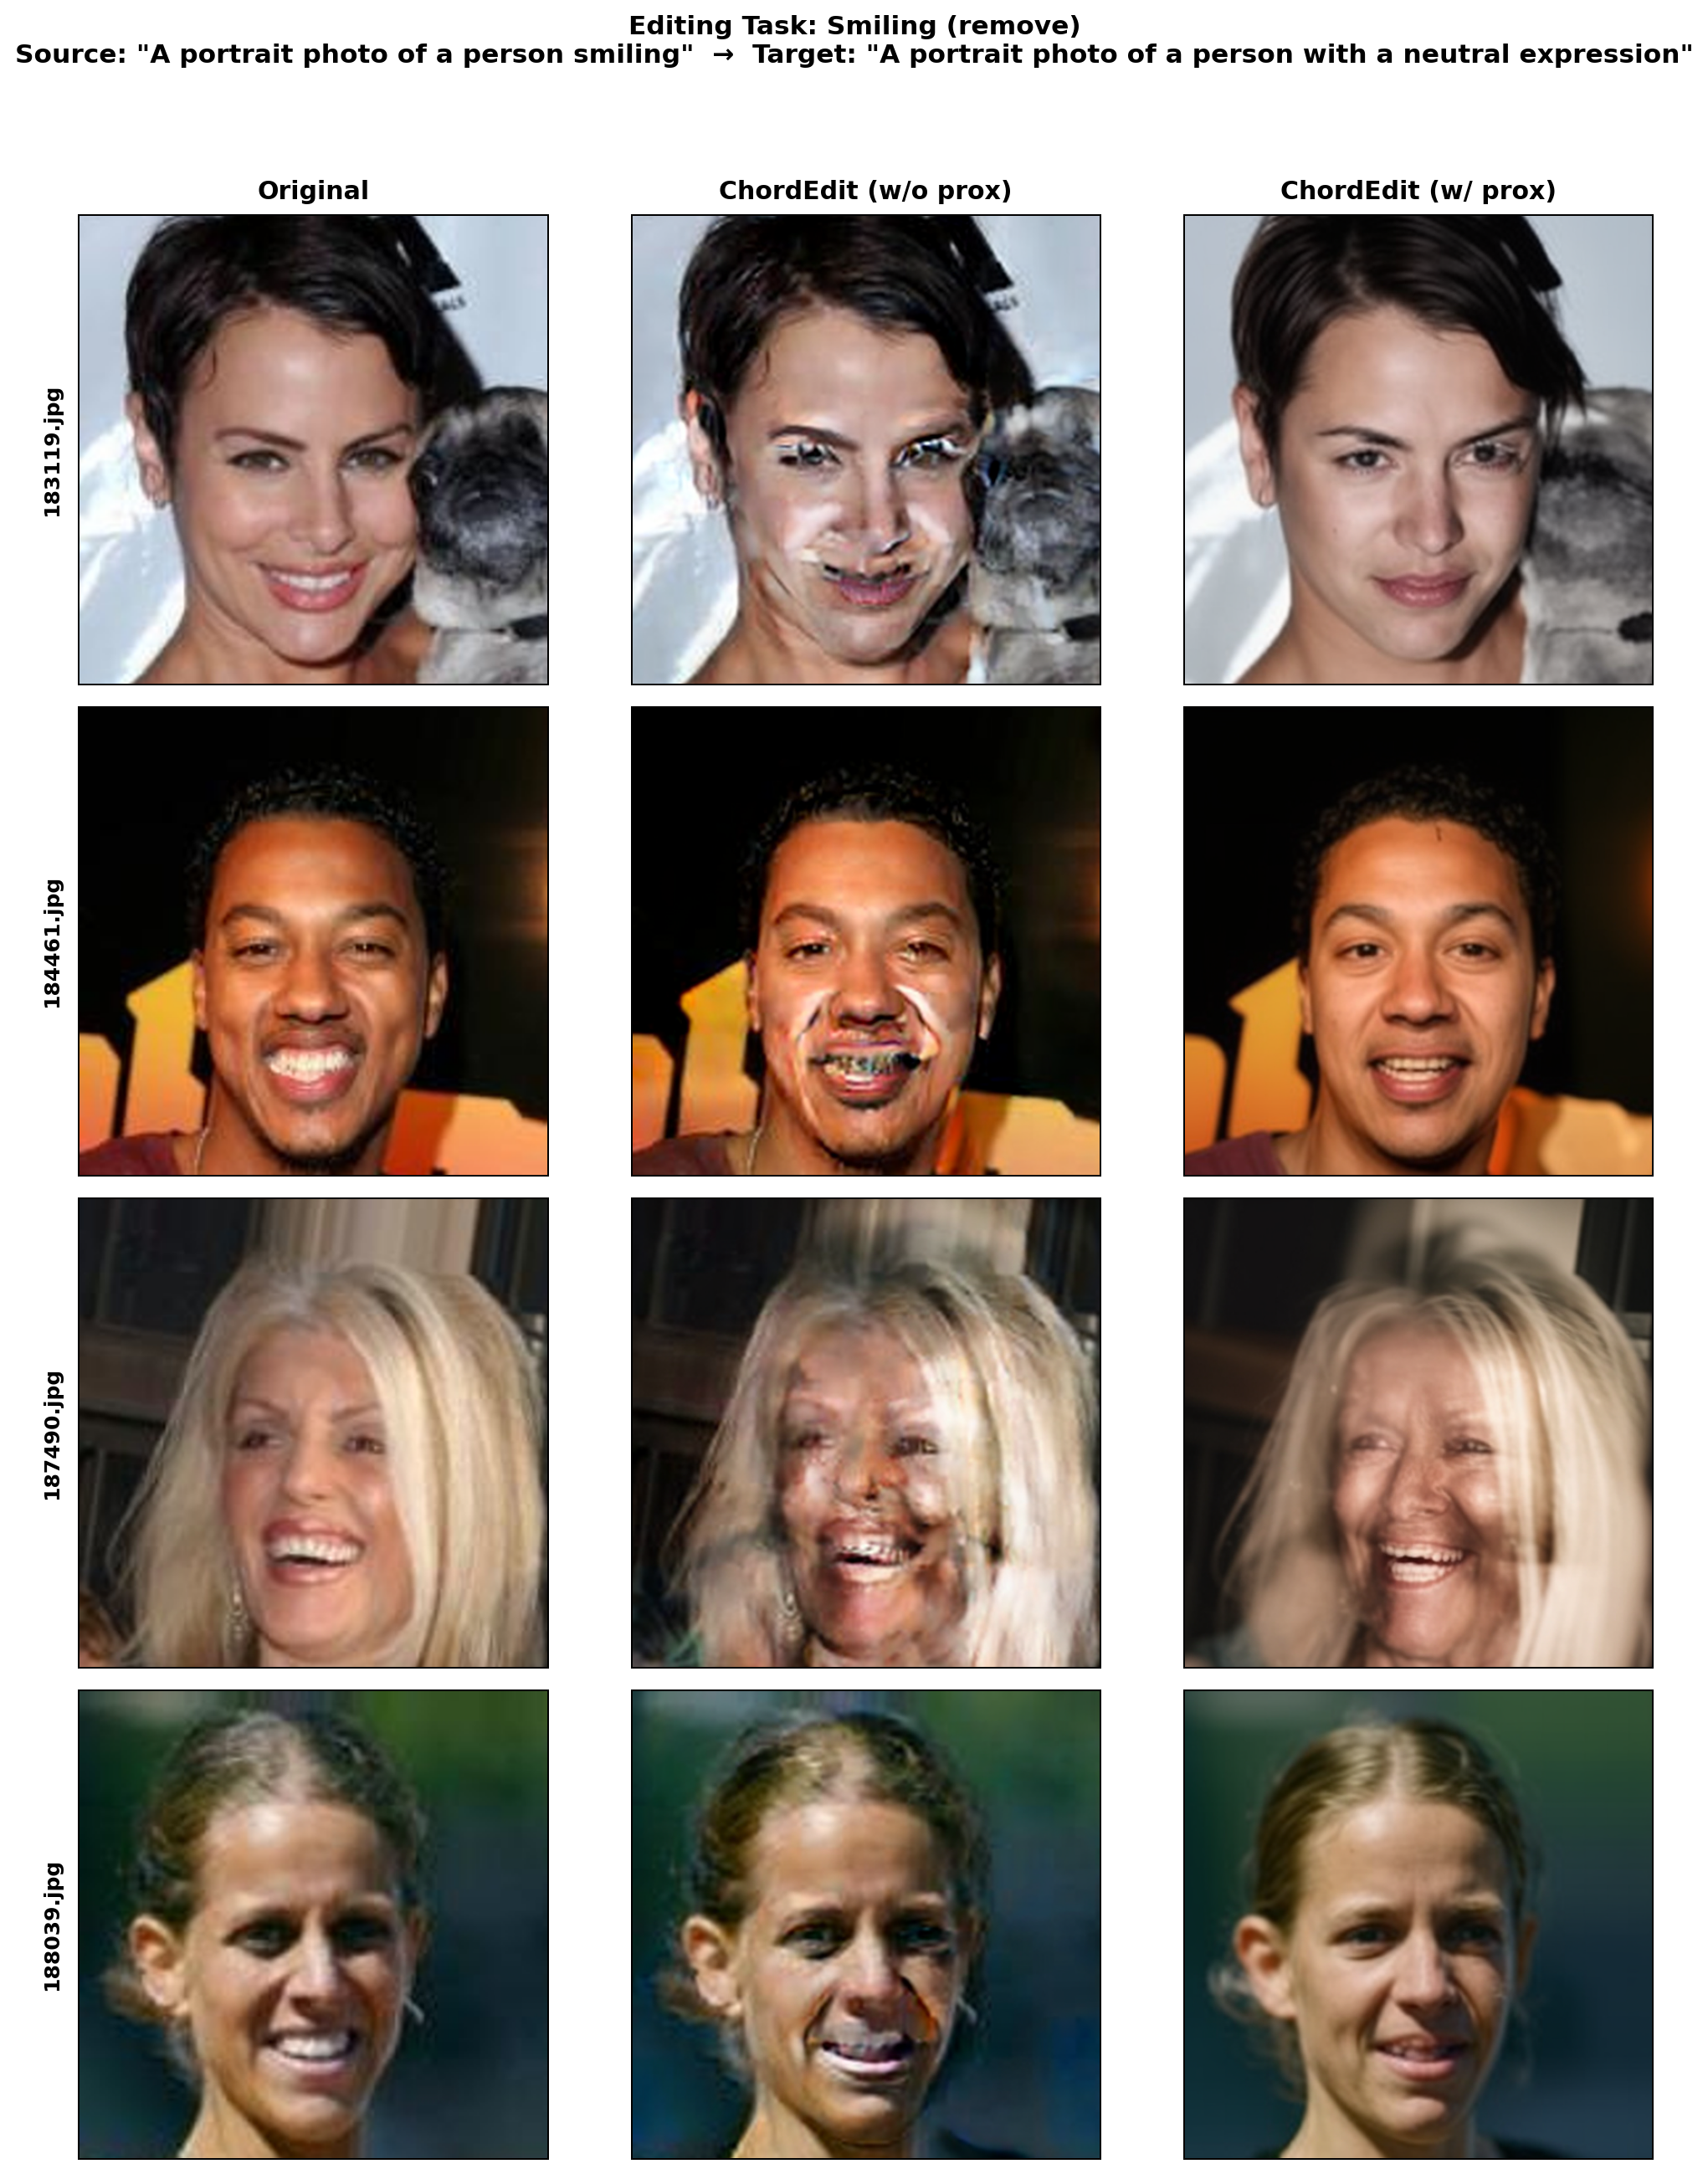
\includegraphics[width=0.95\textwidth,height=0.86\textheight,keepaspectratio]{figures/figure_smiling_remove.png}
    \caption{Qualitative baseline results for \textbf{Smiling (\texttt{remove})}: comparing Original, ChordEdit (w/o prox), and ChordEdit (w/ prox).}
    \label{fig:smiling_remove}
\end{figure}

\begin{figure}[p]
    \centering
    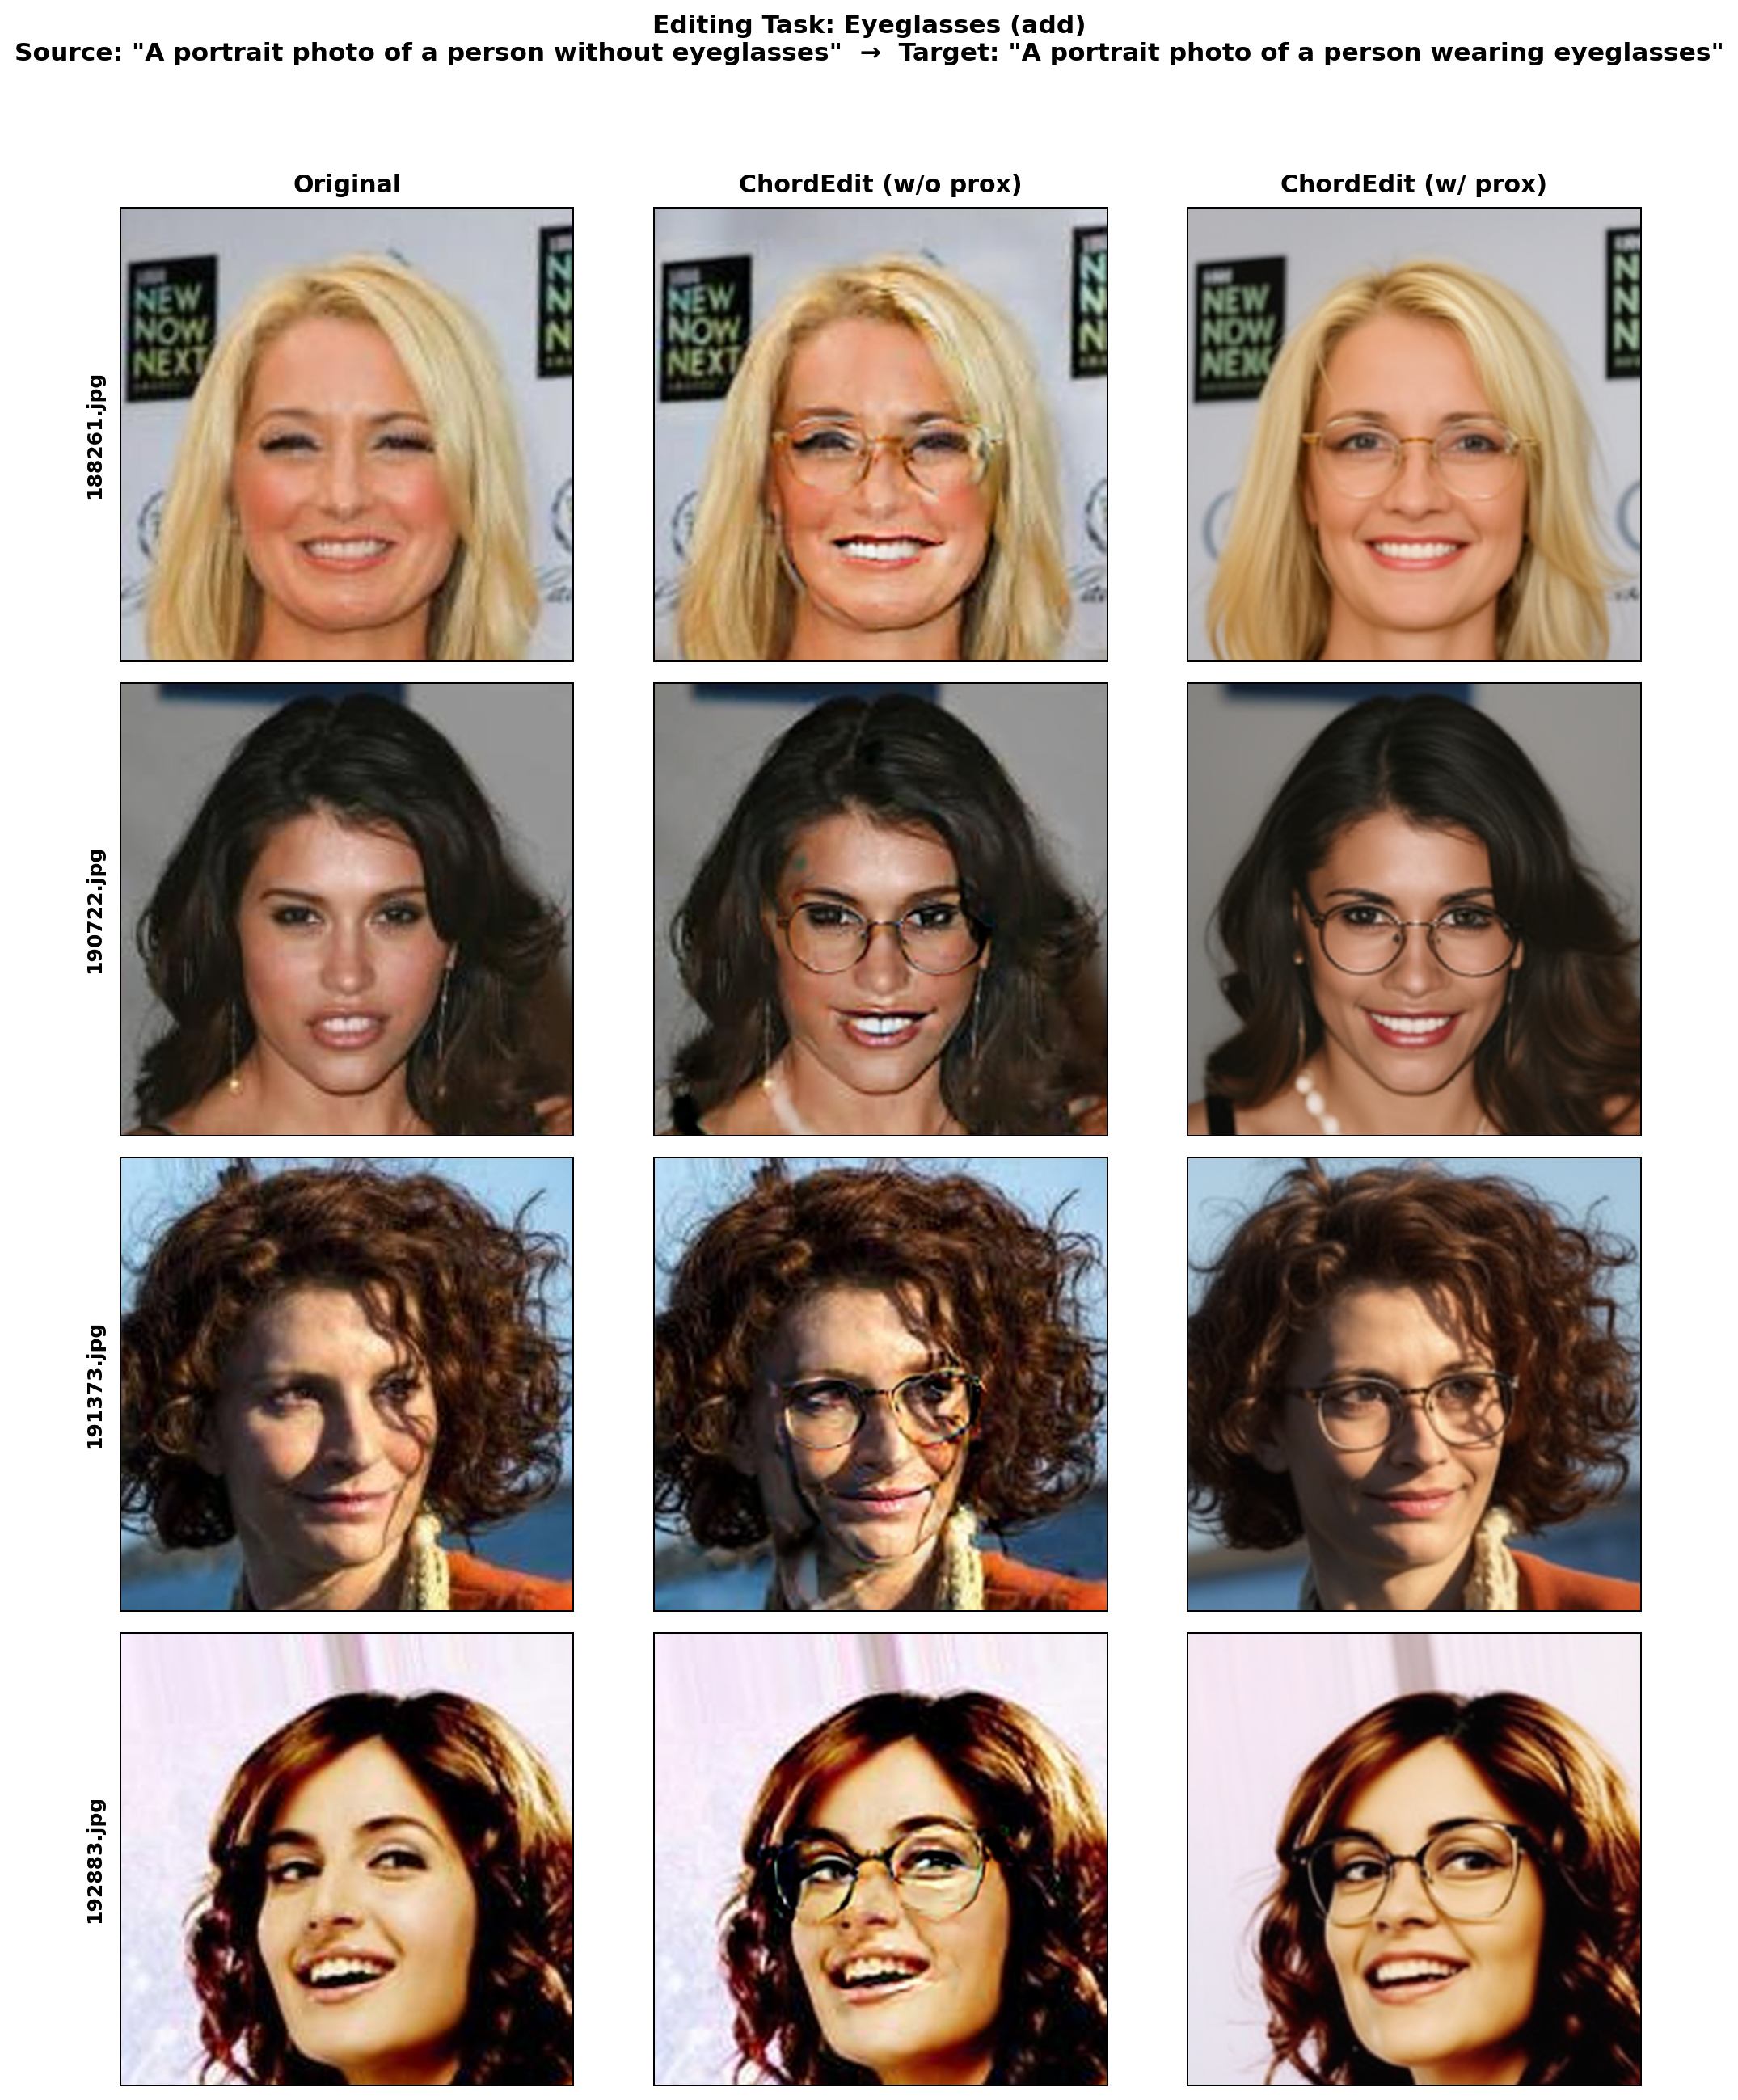
\includegraphics[width=0.95\textwidth,height=0.86\textheight,keepaspectratio]{figures/figure_eyeglasses_add.png}
    \caption{Qualitative baseline results for \textbf{Eyeglasses (\texttt{add})}: comparing Original, ChordEdit (w/o prox), and ChordEdit (w/ prox).}
    \label{fig:eyeglasses_add}
\end{figure}

\begin{figure}[p]
    \centering
    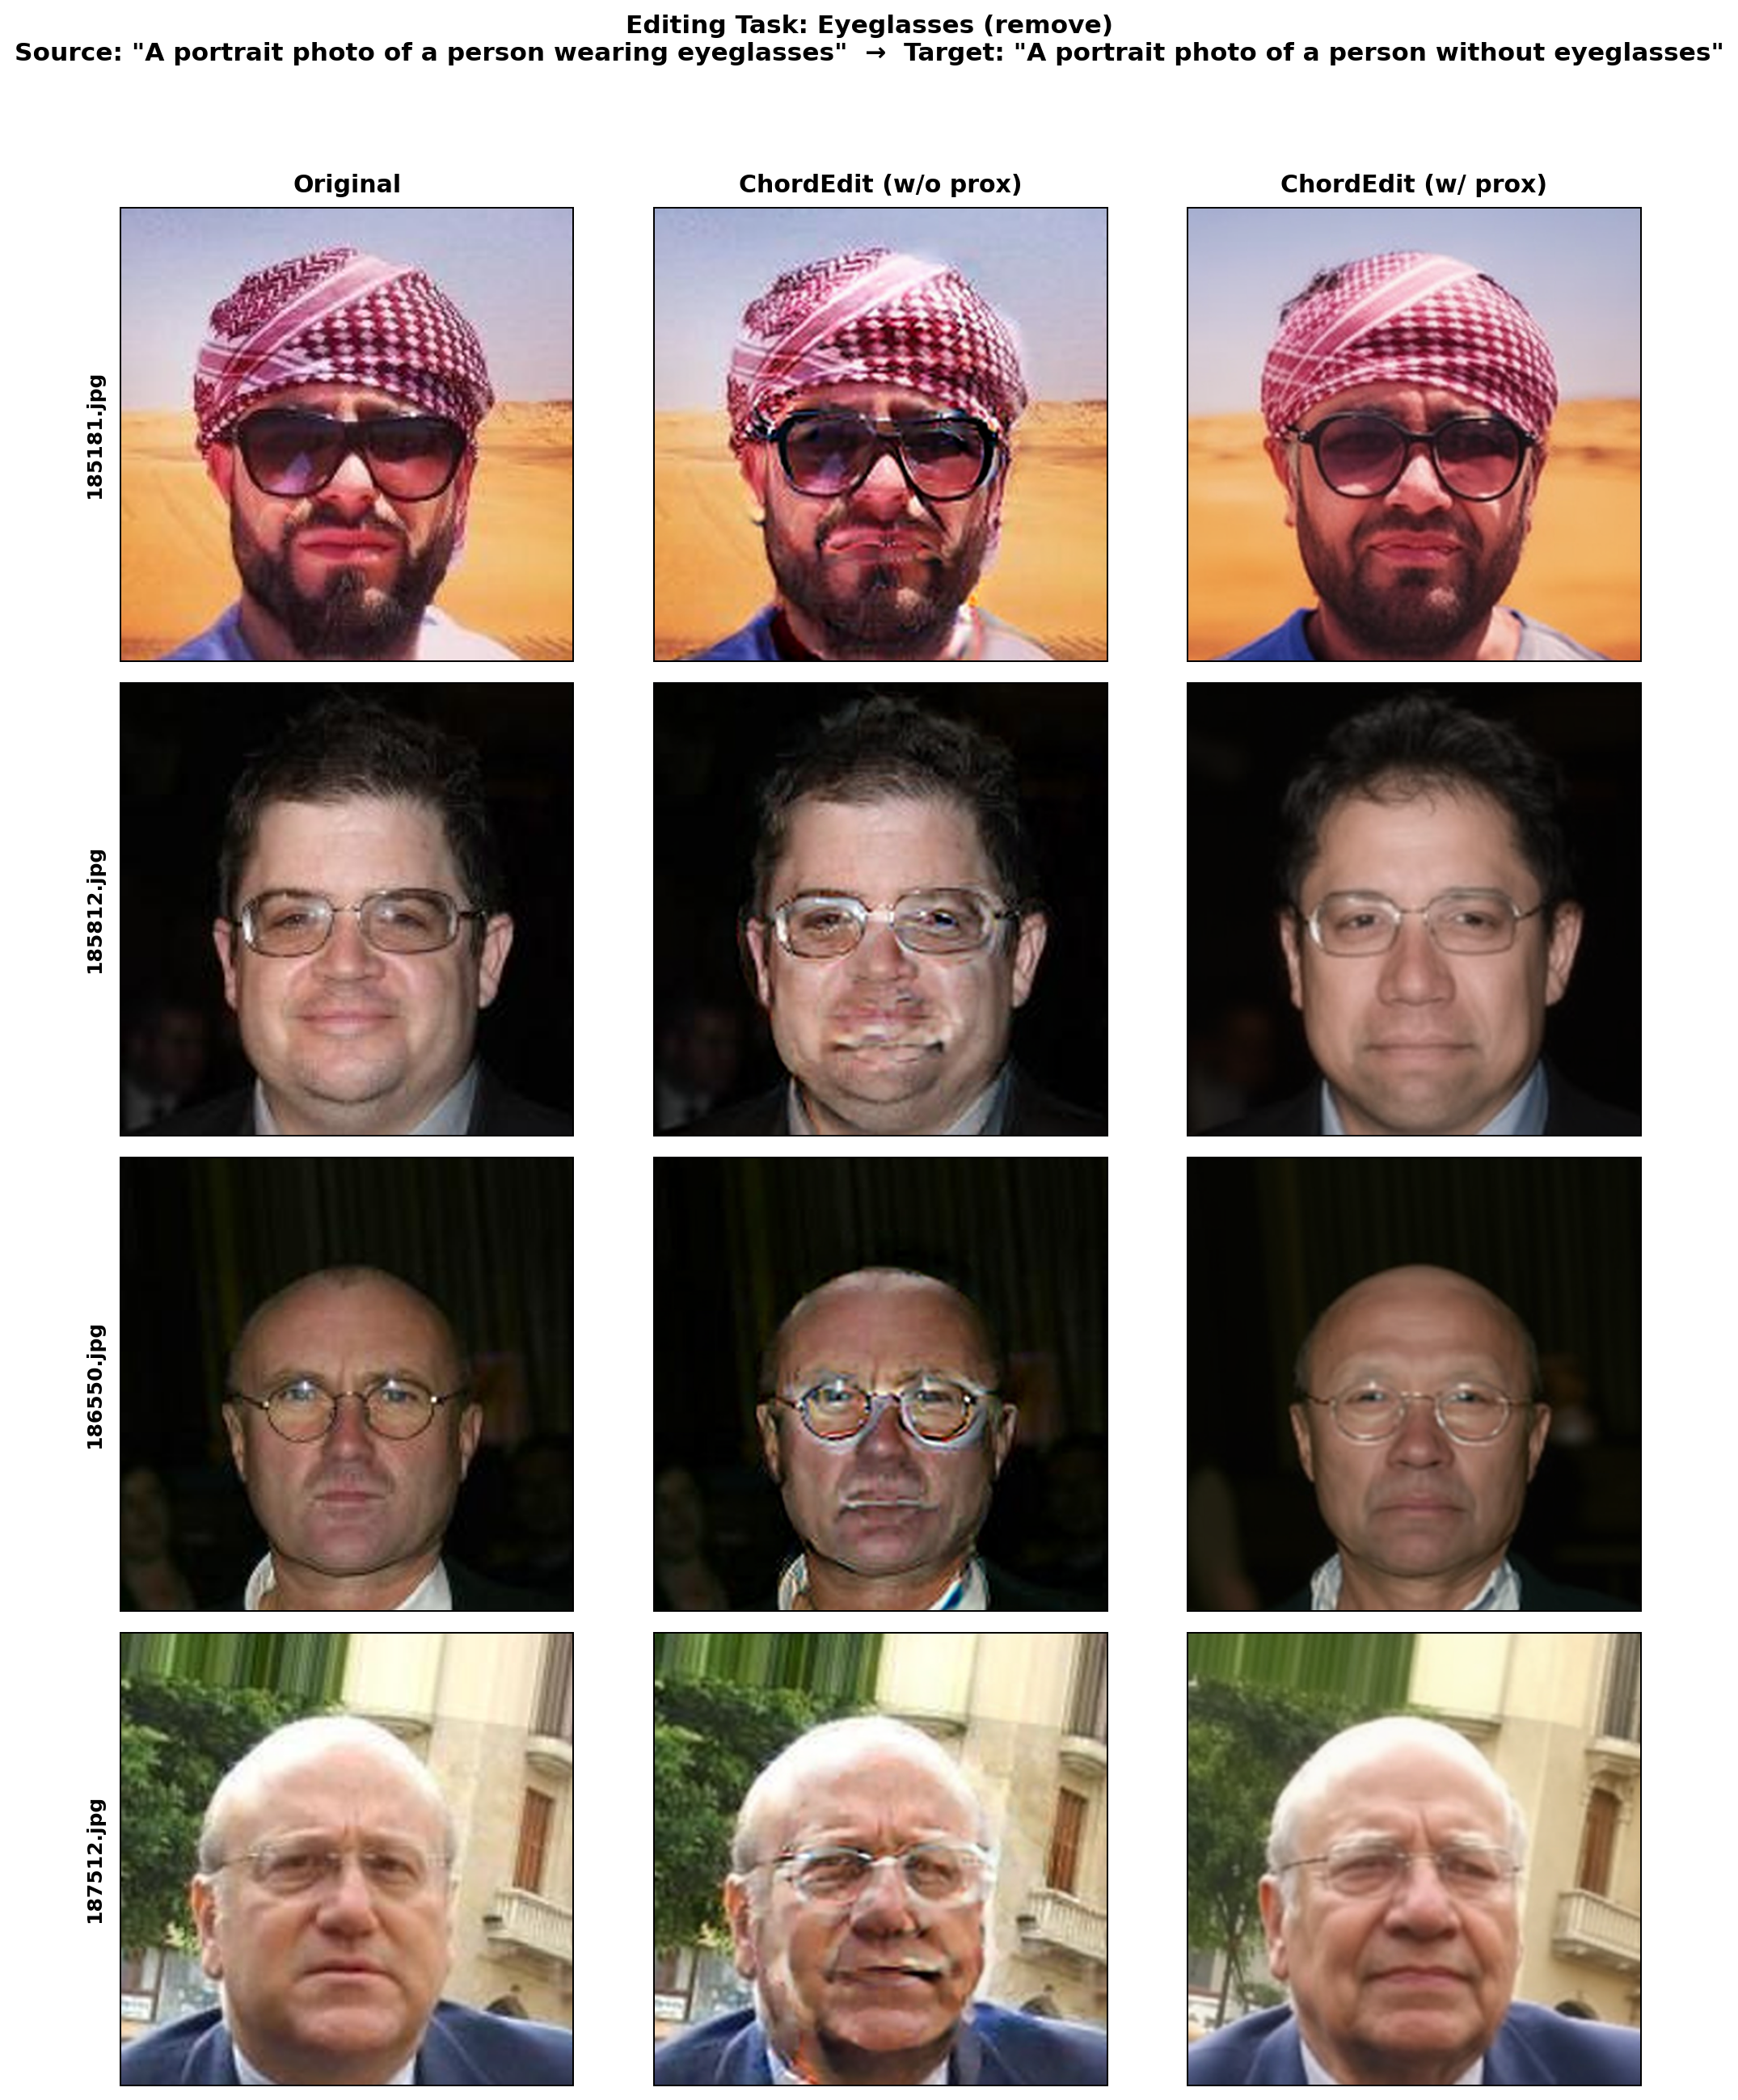
\includegraphics[width=0.95\textwidth,height=0.86\textheight,keepaspectratio]{figures/figure_eyeglasses_remove.png}
    \caption{Qualitative baseline results for \textbf{Eyeglasses (\texttt{remove})}: comparing Original, ChordEdit (w/o prox), and ChordEdit (w/ prox).}
    \label{fig:eyeglasses_remove}
\end{figure}

\begin{figure}[p]
    \centering
    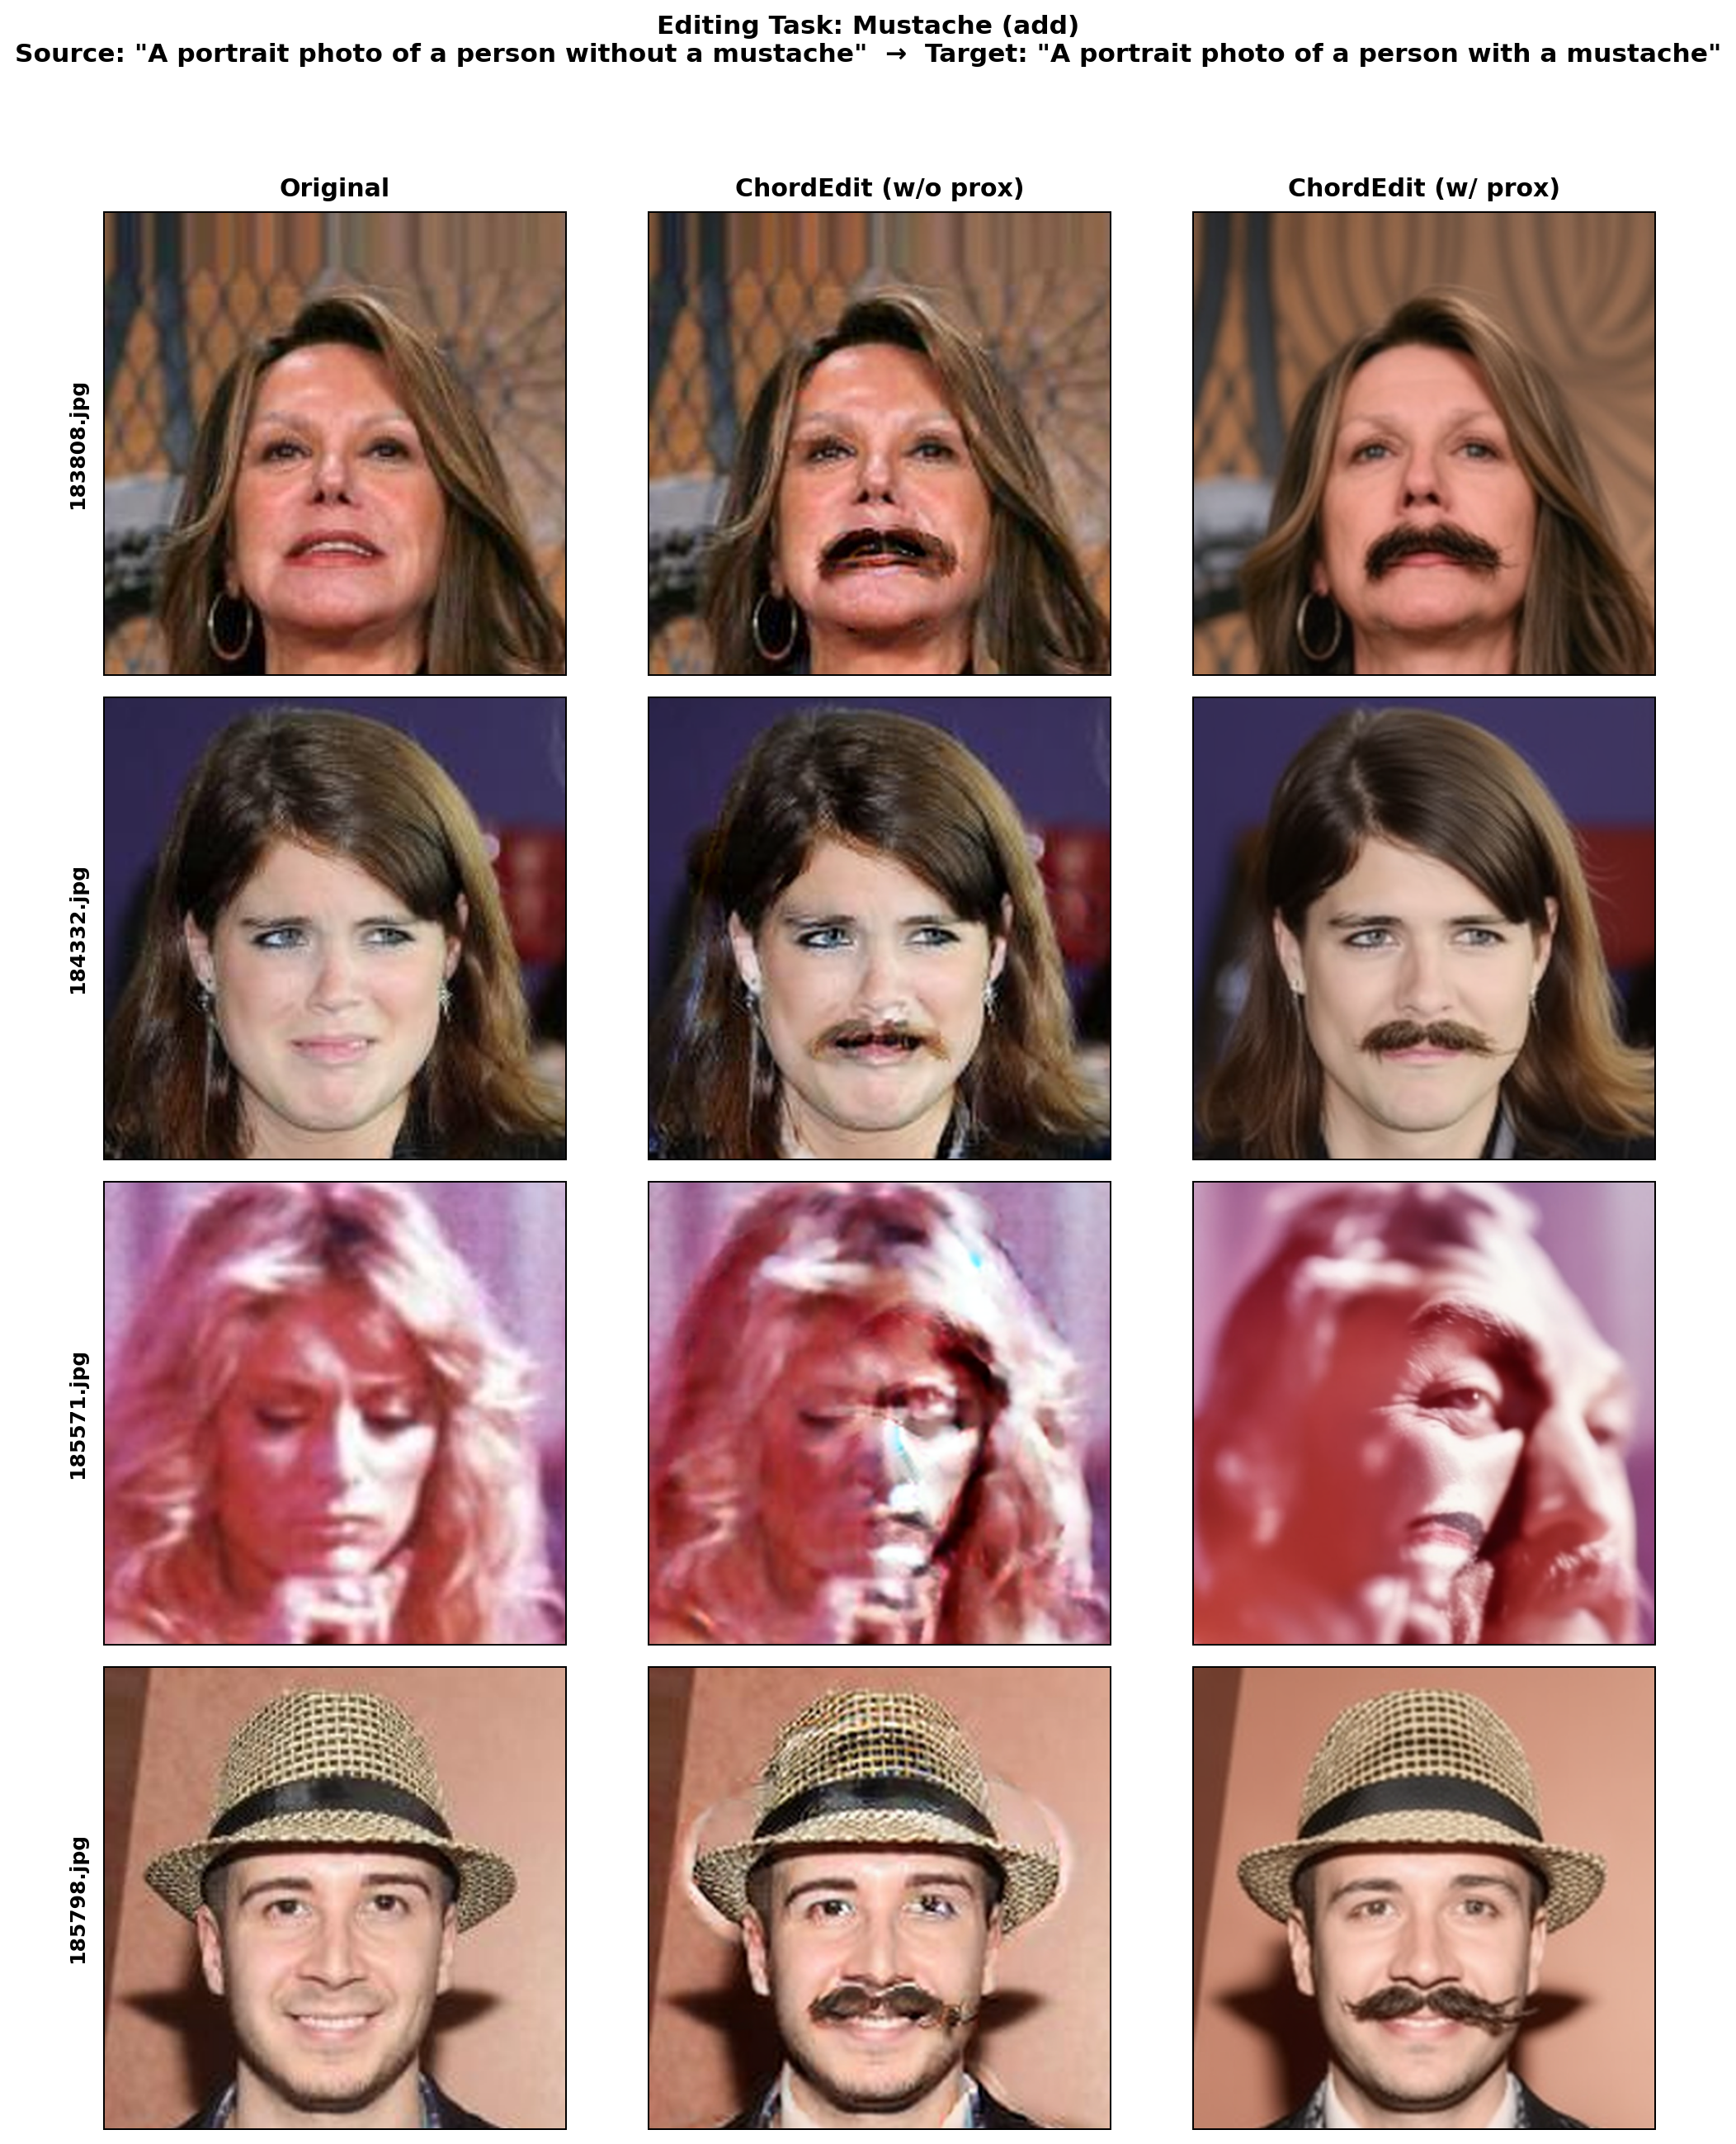
\includegraphics[width=0.95\textwidth,height=0.86\textheight,keepaspectratio]{figures/figure_mustache_add.png}
    \caption{Qualitative baseline results for \textbf{Mustache (\texttt{add})}: comparing Original, ChordEdit (w/o prox), and ChordEdit (w/ prox).}
    \label{fig:mustache_add}
\end{figure}

\begin{figure}[p]
    \centering
    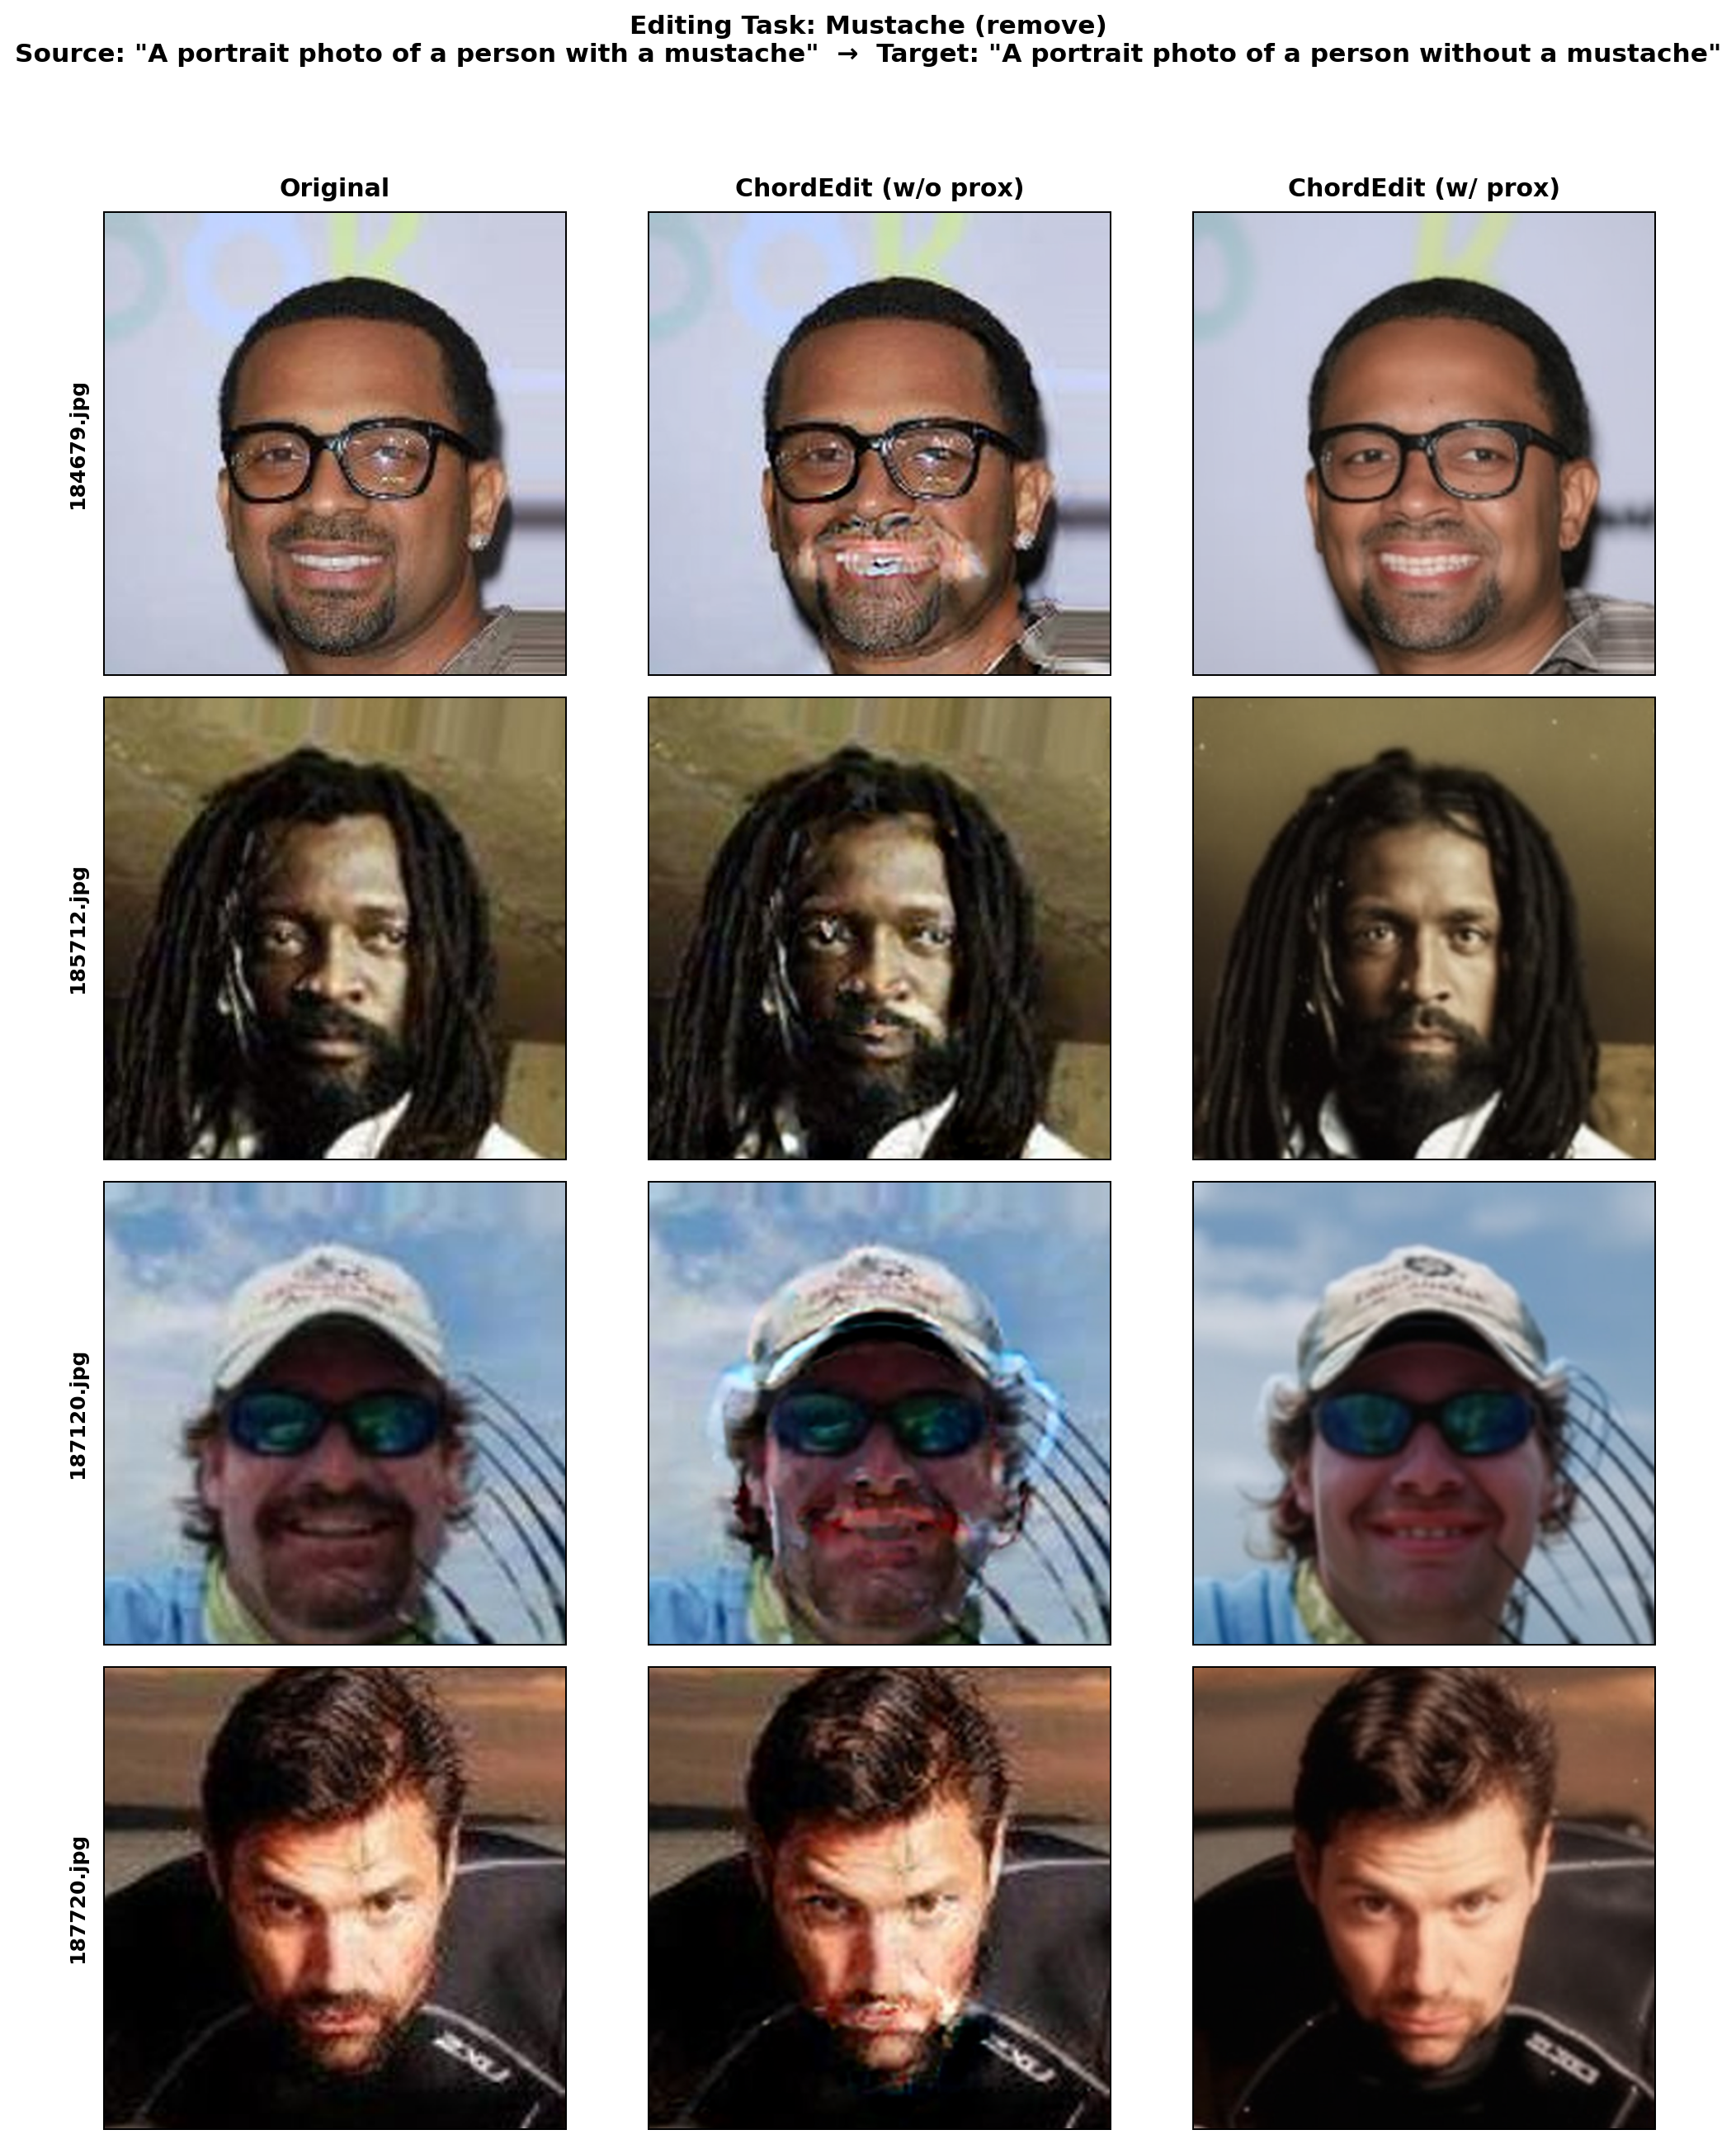
\includegraphics[width=0.95\textwidth,height=0.86\textheight,keepaspectratio]{figures/figure_mustache_remove.png}
    \caption{Qualitative baseline results for \textbf{Mustache (\texttt{remove})}: comparing Original, ChordEdit (w/o prox), and ChordEdit (w/ prox).}
    \label{fig:mustache_remove}
\end{figure}

\clearpage

% ---------------------------------------------------------------------------
% References (Matching 23125001_23125006_23125010_Revised_Proposal.pdf)
% ---------------------------------------------------------------------------
\begin{thebibliography}{12}

\bibitem{lu2026chordedit}
Liangsi Lu, Xuhang Chen, Minzhe Guo, Shichu Li, Jingchao Wang, and Yang Shi.
\newblock ChordEdit: One-step low-energy transport for image editing.
\newblock \emph{arXiv preprint arXiv:2602.19083}, 2026. Version 2, March 25, 2026.

\bibitem{li2026rethinking}
Minghan Li, Jeremy Moebel, and Mengyu Wang.
\newblock Rethinking one-step image editing through ChordEdit: Reproduction, simplification, and new insights.
\newblock \emph{arXiv preprint arXiv:2606.14042}, 2026. Version 1. \url{https://arxiv.org/abs/2606.14042v1}.

\bibitem{choi2018stargan}
Yunjey Choi, Minje Choi, Munyoung Kim, Jung-Woo Ha, Sunghun Kim, and Jaegul Choo.
\newblock StarGAN: Unified generative adversarial networks for multi-domain image-to-image translation.
\newblock In \emph{Proceedings of the IEEE Conference on Computer Vision and Pattern Recognition (CVPR)}, pages 8789--8797, 2018.

\bibitem{liu2019stgan}
Ming Liu, Yukang Ding, Min Xia, Xiao Liu, Errui Ding, Wangmeng Zuo, and Shilei Wen.
\newblock STGAN: A unified selective transfer network for arbitrary image attribute editing.
\newblock In \emph{Proceedings of the IEEE/CVF Conference on Computer Vision and Pattern Recognition (CVPR)}, pages 3673--3682, 2019.

\bibitem{xu2024infedit}
Sihan Xu, Yidong Huang, Jiayi Pan, Ziqiao Ma, and Joyce Chai.
\newblock Inversion-free image editing with language-guided diffusion models.
\newblock In \emph{Proceedings of the IEEE/CVF Conference on Computer Vision and Pattern Recognition (CVPR)}, pages 9452--9461, 2024.

\bibitem{kulikov2025flowedit}
Vladimir Kulikov, Matan Kleiner, Inbar Huberman-Spiegelglas, and Tomer Michaeli.
\newblock FlowEdit: Inversion-free text-based editing using pre-trained flow models.
\newblock In \emph{Proceedings of the IEEE/CVF International Conference on Computer Vision (ICCV)}, pages 19721--19730, 2025.

\bibitem{chordedit_repo}
ChordEdit Authors.
\newblock ChordEdit: Official implementation.
\newblock Official GitHub repository, 2026. Accessed October 27, 2026.

\bibitem{sdturbo}
Stability AI.
\newblock SD-Turbo model card.
\newblock \url{https://huggingface.co/stabilityai/sd-turbo}. Accessed October 27, 2026.

\bibitem{radford2021clip}
Alec Radford, Jong Wook Kim, Chris Hallacy, Aditya Ramesh, Gabriel Goh, Sandhini Agarwal, Girish Sastry, Amanda Askell, Pamela Mishkin, Jack Clark, Gretchen Krueger, and Ilya Sutskever.
\newblock Learning transferable visual models from natural language supervision.
\newblock In \emph{Proceedings of the 38th International Conference on Machine Learning (ICML)}, volume 139 of \emph{Proceedings of Machine Learning Research}, pages 8748--8763, 2021.

\bibitem{liu2015celeba}
Ziwei Liu, Ping Luo, Xiaogang Wang, and Xiaoou Tang.
\newblock Deep learning face attributes in the wild.
\newblock In \emph{Proceedings of the IEEE International Conference on Computer Vision (ICCV)}, pages 3730--3738, 2015.

\bibitem{celeba_web}
Multimedia Laboratory, The Chinese University of Hong Kong.
\newblock Large-scale CelebFaces attributes (CelebA) dataset.
\newblock Official dataset page and usage agreement. Accessed October 27, 2026.

\bibitem{deng2019arcface}
Jiankang Deng, Jia Guo, Niannan Xue, and Stefanos Zafeiriou.
\newblock ArcFace: Additive angular margin loss for deep face recognition.
\newblock In \emph{Proceedings of the IEEE/CVF Conference on Computer Vision and Pattern Recognition (CVPR)}, pages 4690--4699, 2019.

\end{thebibliography}

\end{document}
